%\documentclass[serif, mathserif, professionalfont]{beamer}
\documentclass[13pt,aspectratio=1610]{beamer}
%\usetheme{BlueGrey}
%\usenavigationsymbolstemplate{}
%\usetheme[
%        menuwidth={0.3\paperwidth}
%        ]{amznbln}

\setbeamercovered{transparent=20}

\setlength{\parskip}{0.05cm}

\setlength{\parskip}{1em}

%\documentclass{beamer}



\usepackage{algorithmic,multirow,colortbl}
\usepackage{animate}
\usepackage{tikz}
\usepackage{natbib}
\newcommand{\tikzmark}[1]{\tikz[overlay, remember picture] \coordinate (#1);}
\usepackage{appendixnumberbeamer}

%\usetheme[
%        menuwidth={0.3\paperwidth}
 %       ]{amznbln}

%\setbeamercolor{framesubtitle}{fg=red}
%\addtobeamertemplate{frametitle}{}{%
%  \ifx\insertframesubtitle\@empty\else%
%  \usebeamerfont{framesubtitle}%
%  \usebeamercolor[fg]{framesubtitle}%
%  \insertframesubtitle%
%  \fi%
%}

\setbeamercovered{transparent=20}
% This file defines macros, notation is defined in notationDef.tex
\usepackage{color}
\usepackage{verbatim}

\global\long\def\neil#1{\textbf{\color{red}#1}}
%\global\long\def\todo#1{\textbf{TODO: #1}}
\global\long\def\instructions#1{\textbf{INSTRUCTIONS: #1}}

\definecolor{brown}{rgb}{0.9,0.59,0.078}
\definecolor{ironsulf}{rgb}{0,0.7,.5}
\definecolor{lightpurple}{rgb}{0.156,0,0.245}

\newenvironment{matlab}{\comment}{\endcomment}
\newenvironment{octave}{\comment}{\endcomment}
\newenvironment{matlabv}{\verbatim}{\endverbatim}
\newenvironment{octavev}{\verbatim}{\endverbatim}

\ifdefined\blackBackground
\definecolor{colorOne}{rgb}{0, 1, 1}
\definecolor{colorTwo}{rgb}{1, 0, 1}
\definecolor{colorThree}{rgb}{1, 1, 0}
\definecolor{colorTwoThree}{rgb}{1, 0, 0}
\definecolor{colorOneThree}{rgb}{0, 1, 0}
\definecolor{colorOneTwo}{rgb}{0, 0, 1}
\else
\definecolor{colorOne}{rgb}{1, 0, 0}
\definecolor{colorTwo}{rgb}{0, 1, 0}
\definecolor{colorThree}{rgb}{0, 0, 1}
\definecolor{colorTwoThree}{rgb}{0, 1, 1}
\definecolor{colorOneThree}{rgb}{1, 0, 1}
\definecolor{colorOneTwo}{rgb}{1, 1, 0}
\fi

\ifdefined\blackBackground
\global\long\def\redColor{cyan}
\global\long\def\greenColor{magenta}
\global\long\def\blueColor{yellow}
\global\long\def\magentaColor{green}
\global\long\def\blackColor{white}
\global\long\def\whiteColor{black}
\else
\global\long\def\redColor{red}
\global\long\def\greenColor{green}
\global\long\def\blueColor{blue}
\global\long\def\magentaColor{magenta}
\global\long\def\blackColor{black}
\global\long\def\whiteColor{white}
\fi

\global\long\def\det#1{\left|#1\right|}
\global\long\def\erf{\text{erf}}
\global\long\def\refeq#1{(\ref{#1})}
\global\long\def\refsec#1{Section \ref{#1}}
\global\long\def\refsecs#1#2{Sections \ref{#1}--\ref{#2}}
\global\long\def\reftwosec#1#2{Sections \ref{#1} and \ref{#2}}
\global\long\def\Refsec#1{Section \ref{#1}}

% Try and avoid these macros for notation, they are definitions of convenience.
\global\long\def\bfdelta{\boldsymbol{\delta}}
\global\long\def\bfDelta{\boldsymbol{\Delta}}
\global\long\def\bfbeta{\boldsymbol{\beta}}
\global\long\def\bfgamma{\boldsymbol{\gamma}}
\global\long\def\bfmu{\boldsymbol{\mu}}
\global\long\def\bfnu{\boldsymbol{\nu}}
\global\long\def\bfalpha{\boldsymbol{\alpha}}
\global\long\def\bfepsilon{\boldsymbol{\epsilon}}
\global\long\def\bfSigma{\boldsymbol{\Sigma}}
\global\long\def\bftau{\boldsymbol{\tau}}
\global\long\def\bflambda{\boldsymbol{\lambda}}
\global\long\def\bfLambda{\boldsymbol{\Lambda}}
\global\long\def\bfpsi{\boldsymbol{\psi}}
\global\long\def\bfxi{\boldsymbol{\xi}}
\global\long\def\bfpi{\bm{\pi}}
\global\long\def\bfPsi{\boldsymbol{\Psi}}
\global\long\def\bfphi{\boldsymbol{\phi}}
\global\long\def\bfPhi{\boldsymbol{\Phi}}
\global\long\def\bfrho{\boldsymbol{\rho}}
\global\long\def\bftheta{\boldsymbol{\theta}}
\global\long\def\bfTheta{\boldsymbol{\Theta}}
\global\long\def\bfomega{\boldsymbol{\omega}}


\global\long\def\Bmath#1{\boldsymbol{#1}}


% Avoid these macros for notation, they are definitions of convenience.
\global\long\def\bfa{\mathbf{a}}
\global\long\def\bfb{\mathbf{b}}
\global\long\def\bfc{\mathbf{c}}
\global\long\def\bfd{\mathbf{d}}
\global\long\def\bfe{\mathbf{e}}
\global\long\def\bff{\mathbf{f}}
\global\long\def\bfg{\mathbf{g}}
\global\long\def\bfh{\mathbf{h}}
\global\long\def\bfk{\mathbf{k}}
\global\long\def\bfl{\mathbf{l}}
\global\long\def\bfm{\mathbf{m}}
\global\long\def\bfn{\mathbf{n}}
\global\long\def\bfo{\mathbf{o}}
\global\long\def\bfp{\mathbf{p}}
\global\long\def\bfq{\mathbf{q}}
\global\long\def\bfr{\mathbf{r}}
\global\long\def\bfs{\mathbf{s}}
\global\long\def\bft{\mathbf{t}}
\global\long\def\bfu{\mathbf{u}}
\global\long\def\bfv{\mathbf{v}}
\global\long\def\bfw{\mathbf{w}}
\global\long\def\bfx{\mathbf{x}}
\global\long\def\bfy{\mathbf{y}}
\global\long\def\bfz{\mathbf{z}}

\newcommand{\dif}[1]{\text{d}#1}
\global\long\def\cov{\text{cov}}


\global\long\def\bfzero{\mathbf{0}}
\global\long\def\bfone{\mathbf{1}}


\global\long\def\bfA{\mathbf{A}}
\global\long\def\bfB{\mathbf{B}}
\global\long\def\bfC{\mathbf{C}}
\global\long\def\bfD{\mathbf{D}}
\global\long\def\bfE{\mathbf{E}}
\global\long\def\bfG{\mathbf{G}}
\global\long\def\bfH{\mathbf{H}}
\global\long\def\bfI{\mathbf{I}}
\global\long\def\eye{\mathbf{I}}
\global\long\def\bfK{\mathbf{K}}
\global\long\def\bfL{\mathbf{L}}
\global\long\def\bfM{\mathbf{M}}
\global\long\def\bfO{\mathbf{O}}
\global\long\def\bfP{\mathbf{P}}
\global\long\def\bfQ{\mathbf{Q}}
\global\long\def\bfR{\mathbf{R}}
\global\long\def\bfS{\mathbf{S}}
\global\long\def\bfT{\mathbf{T}}
\global\long\def\bfU{\mathbf{U}}
\global\long\def\bfV{\mathbf{V}}
\global\long\def\bfW{\mathbf{W}}
\global\long\def\bfX{\mathbf{X}}
\global\long\def\bfY{\mathbf{Y}}
\global\long\def\bfZ{\mathbf{Z}}
\global\long\def\llangle{{\langle\vspace{-2mm} \langle}}
\global\long\def\rrangle{{\rangle\vspace{-2mm} \rangle}}
\global\long\def\la{\leftarrow}


\global\long\def\tf{\tilde{f}}
\global\long\def\tg{\tilde{g}}
\global\long\def\tX{\tilde{X}}
\global\long\def\tY{\tilde{Y}}
\global\long\def\tZ{\tilde{Z}}


\global\long\def\bbE{\mathbb{E}}
\global\long\def\bbR{\mathbb{R}}
\global\long\def\bbP{\mathbb{P}}
\global\long\def\bbT{\mathbb{T}}
\global\long\def\bbZ{\mathbb{Z}}


\global\long\def\ois{2 \pi i s}
\global\long\def\oik{2 \pi i k}
\global\long\def\oin{2 \pi i n}
\global\long\def\oim{2 \pi i m}


\global\long\def\T{{\top}}
\global\long\def\Tr{\mbox{Tr}}
\global\long\def\trace#1{\text{tr}\left(#1\right)}
%\global\long\def\diff#1{{\, d#1}}
\global\long\def\diff#1#2{\frac{\text{d}#1}{\text{d}#2}}
\global\long\def\vgraph#1{ \newpage\begin{center} \end{center}{center}{center}{center}{center}{center}{center}{center}{center}{center}{center}{center}{center}{center}{center}{center}{center} {\large{\bf #1}} {center} \vspace{2mm} }
\global\long\def\high#1{\textcolor{blue}{\emph{#1}}}
\global\long\def\cut#1{}
\global\long\def\citeasnoun#1{\citeN{#1}}
\global\long\def\citemulti#1#2{(#1, \citeyearNP{#2})}
\global\long\def\citemultiN#1#2{#1 (\citeyearNP{#2})}
\global\long\def\Sum{{\displaystyle \sum}}
\global\long\def\defeq{{\stackrel{def}{=}}}
\global\long\def\marg#1{\marginpar{#1}}


\global\long\def\pdt#1#2{\frac{\partial^{2} #1}{\partial{#2}^{2} }}
\global\long\def\pdsd#1#2#3{\frac{\partial^{2} #1}{\partial{#2} \partial{#3} }}
\global\long\def\pdo#1#2{\frac{\partial{#1}}{\partial{#2}}}
\global\long\def\pdol#1#2{\partial{#1}/ \partial{#2}}
\global\long\def\pdu#1{\frac{\partial}{\partial{#1}}}

\global\long\def\reffig#1{figure~\ref{#1}}
\global\long\def\Reffig#1{Figure~\ref{#1}}
\global\long\def\reffigrange#1#2{figure~\ref{#1}--\ref{#2}}
\global\long\def\Reffigrange#1#2{Figure~\ref{#1}--\ref{#2}}
\global\long\def\refbox#1{box~\ref{#1}}
\global\long\def\Refbox#1{Box~\ref{#1}}
\global\long\def\refeqs#1#2{equation~(\ref{#1})--(\ref{#2})}
\global\long\def\Refeqs#1#2{Equation~(\ref{#1})--(\ref{#2})}
\global\long\def\reftip#1{tip~\ref{#1}}
\global\long\def\Reftip#1{Tip~\ref{#1}}
\global\long\def\refint#1{intuition~\ref{#1}}
\global\long\def\Refint#1{Intuition~\ref{#1}}
\global\long\def\reftable#1{table~\ref{#1}}
\global\long\def\Reftable#1{Table~\ref{#1}}
\global\long\def\refchap#1{chapter~\ref{#1}}
\global\long\def\Refchap#1{Chapter~\ref{#1}}
\global\long\def\refapp#1{appendix~\ref{#1}}
\global\long\def\Refappendix#1{Appendix~\ref{#1}}
\global\long\def\refchaprange#1#2{chapter~\ref{#1}--\ref{#2}}
\global\long\def\Refchaprange#1#2{Chapter~\ref{#1}--\ref{#2}}
\global\long\def\refsection#1{section~\ref{#1}}
\global\long\def\Refsection#1{Section~\ref{#1}}

\global\long\def\fixme#1{\emph{\textbf{#1}}}

\global\long\def\detail#1{}

% For putting a footer when an include is made.
\global\long\def\includetalkfile#1{{\setbeamertemplate{footline}{\url{#1} \hfill \insertframenumber} \input{#1}}}

%\global\long\def\includetalkfile#1{\input{#1}}
\global\long\def\newsection#1#2{\section{#1}\begin{frame}\frametitle{Outline}\tableofcontents[currentsection,hideallsubsections]\end{frame}\includetalkfile{#2}}

\global\long\def\inputdiagram#1{{\small\input{#1}\vspace{0.5cm}}}

\global\long\def\newsubsection#1#2{\subsection{#1}\includetalkfile{#2}}
\global\long\def\newsubsubsection#1#2{\subsubsection{#1}\includetalkfile{#2}}


\global\long\def\includeyoutube#1{\includemedia[
  width=0.6\linewidth,height=0.45\linewidth,
  activate=pageopen,
  flashvars={
    modestbranding=1 % no YT logo in control bar
   &autohide=1       % controlbar autohide
   &showinfo=0       % no title and other info before start
  }
]{}{https://www.youtube.com/v/#1?rel=0}}

\global\long\def\includesmallyoutube#1{\includemedia[
  width=0.4\linewidth,height=0.3\linewidth,
  activate=pageopen,
  flashvars={
    modestbranding=1 % no YT logo in control bar
   &autohide=1       % controlbar autohide
   &showinfo=0       % no title and other info before start
  }
]{}{https://youtube.googleapis.com/v/#1?rel=0}}


\global\long\def\includevimeo#1{\includemedia[width=0.6\linewidth,height=0.45\linewidth,activate=pageopen]{}{http://vimeo.com/moogaloop.swf?clip_id=#1}}

\global\long\def\includecvfile#1{\input{#1}}
\global\long\def\newcvsection#1#2{\section*{#1}\includecvfile{#2}}

\global\long\def\newcvsubsection#1#2{\subsection*{#1}\includecvfile{#2}}
\global\long\def\newcvsubsubsection#1#2{\subsubsection*{#1}\includecvfile{#2}}
\global\long\def\newcvparagraph#1#2{\paragraph{#1}\includecvfile{#2}}

\global\long\def\twoimageslidewidth#1#2#3#4{\begin{frame}[plain]
  \begin{center}
    \href{#3}{\includegraphics[width=0.45\textwidth]{#1}}\hfill
    \href{#3}{\includegraphics[width=0.45\textwidth]{#2}}
  \end{center}
\end{frame}
\note{#4}}
\global\long\def\imageslidewidth#1#2#3{\begin{frame}[plain]
  \begin{center}
    \href{#2}{\includegraphics[width=0.9\textwidth]{#1}}
  \end{center}
\end{frame}
\note{#3}}
\global\long\def\imageslideheight#1#2#3{\begin{frame}[plain]
  \begin{center}
    \href{#2}{\includegraphics[height=0.9\textheight]{#1}}
  \end{center}
\end{frame}
\note{#3}}

\global\long\def\paperslide#1#2#3{\begin{frame}[plain]
  \begin{center}
    {\setlength\fboxsep{0pt}%
      \colorbox{white}{
    \href{#2}{\includegraphics[trim=0cm 20cm 0cm 0cm, clip=true, width=\textwidth]{#1}}}
    }
  \end{center}
\end{frame}
\note{#3}}



% This file defines notation to be used
\global\long\def\outputIndex{j}
\global\long\def\dataIndex{i}
\global\long\def\dataIndexTwo{j}
\global\long\def\latentIndex{j}

\global\long\def\inputSpace{\mathcal{X}}

\global\long\def\conditionalCovariance{\boldsymbol{\Sigma}}

\global\long\def\fantasyDim{r}
\global\long\def\dataDim{p}
\global\long\def\latentDim{q}
\global\long\def\inputDim{q}
\global\long\def\numLayers{\ell}
\global\long\def\numData{n}
\global\long\def\numTime{T}
\global\long\def\numTasks{m}
\global\long\def\numSequences{s}
\global\long\def\numInducing{m}
\global\long\def\numNeighbors{K}
\global\long\def\numHidden{h}
\global\long\def\numComponents{m}
\global\long\def\numBasisFunc{m}
\global\long\def\iterNum{k}
\global\long\def\maxIters{K}

\global\long\def\rbfWidth{\ell}
\global\long\def\lengthScale{\ell}
\global\long\def\binomProb{\pi}

\global\long\def\dataStd{\sigma}
\global\long\def\featureStd{\varsigma}

\global\long\def\heaviside{H}
\global\long\def\errorFunction{E}
\global\long\def\likelihoodFunction{L}
\global\long\def\likelihoodBound{\mathcal{L}}
\global\long\def\lagrangian{L}

\global\long\def\parameterScalar{\theta}
\global\long\def\parameterVector{\boldsymbol{\parameterScalar}}
\global\long\def\parameterMatrix{\boldsymbol{\Theta}}

\global\long\def\dataScalar{y}
\global\long\def\dataVector{\mathbf{\dataScalar}}
\global\long\def\dataMatrix{\mathbf{\MakeUppercase{\dataScalar}}}

\global\long\def\cdataMatrix{\hat{\dataMatrix}}
\global\long\def\cdataVector{\hat{\dataVector}}
\global\long\def\cdataScalar{\hat{\dataScalar}}

\global\long\def\dataSet{\mathcal{D}}

\global\long\def\bigO{\mathcal{O}}


\global\long\def\switchScalar{s}
\global\long\def\switchVector{\mathbf{\switchScalar}}
\global\long\def\switchMatrix{\mathbf{\MakeUppercase{\switchScalar}}}

\global\long\def\latentScalar{x}
\global\long\def\latentMatrix{\mathbf{\MakeUppercase{\latentScalar}}}
\global\long\def\latentVector{\mathbf{\latentScalar}}

\global\long\def\hiddenScalar{h}
\global\long\def\hiddenMatrix{\mathbf{\MakeUppercase{\hiddenScalar}}}
\global\long\def\hiddenVector{\mathbf{\hiddenScalar}}

\global\long\def\noiseMatrix{\boldsymbol{E}}
\global\long\def\noiseVector{\boldsymbol{\epsilon}}
\global\long\def\noiseScalar{\epsilon}

\global\long\def\fantasyScalar{z}
\global\long\def\fantasyVector{\mathbf{\fantasyScalar}}
\global\long\def\fantasyMatrix{\mathbf{\MakeUppercase{\fantasyScalar}}}

\global\long\def\kernelScalar{k}
\global\long\def\kernelVector{\mathbf{\kernelScalar}}
\global\long\def\kernelMatrix{\mathbf{\MakeUppercase{\kernelScalar}}}

\global\long\def\centeredKernelScalar{b}
\global\long\def\centeredKernelVector{\centeredKernelScalar}
\global\long\def\centeredKernelMatrix{\mathbf{\MakeUppercase{\centeredKernelScalar}}}

\global\long\def\latentForce{f}
\global\long\def\LatentForce{F}
\global\long\def\displacement{x}
\global\long\def\displacementVector{\textbf{\displacement}}
\global\long\def\Displacement{X}
\global\long\def\velocity{v}
\global\long\def\acceleration{a}
\global\long\def\lengthScale{\ell}
\global\long\def\naturalFrequency{\omega}
\global\long\def\sensitivity{s}
\global\long\def\mrnaConcentration{m}
\global\long\def\tfConcentration{p}
\global\long\def\tfMrnaConcentration{f}
\global\long\def\tfVector{{\bf \tfConcentration}}
\global\long\def\weightScalar{w}
\global\long\def\weightVector{{\bf \weightScalar}}
\global\long\def\meanVector{\boldsymbol{\mu}}
\global\long\def\zerosVector{{\bf 0}}
\global\long\def\decayRate{d}
\global\long\def\dampingCoefficient{c}
\global\long\def\mass{m}
\global\long\def\basalRate{b}
\global\long\def\Sensitivity{S}
\global\long\def\DecayRate{D}
\global\long\def\tfDecayRate{\delta}
\global\long\def\DampingCoefficient{C}
\global\long\def\Mass{M}
\global\long\def\BasalRate{B}
\global\long\def\basisFunc{\phi}
\global\long\def\basisFuncVector{\boldsymbol{\basisFunc}}
\global\long\def\numBasisFunc{m}
\global\long\def\numData{n}
\global\long\def\numComps{K}
\global\long\def\dataDim{p}

\global\long\def\inputScalar{x}
\global\long\def\inputMatrix{{\bf \MakeUppercase{\inputScalar}}}
\global\long\def\inputVector{{\bf \inputScalar}}

\global\long\def\parameterScalar{\theta}
\global\long\def\parameterVector{\boldsymbol{\parameterScalar}}

\global\long\def\kernel{\kernelScalar}

\global\long\def\covarianceScalar{c}
\global\long\def\covarianceMatrix{\mathbf{\MakeUppercase{\covarianceScalar}}}
\global\long\def\covarianceVector{\mathbf{\covarianceScalar}}

\global\long\def\croupierScalar{s}
\global\long\def\croupierMatrix{\mathbf{\MakeUppercase{\croupierScalar}}}
\global\long\def\croupierVector{\mathbf{\croupierScalar}}

\global\long\def\coregionalizationScalar{b}
\global\long\def\coregionalizationMatrix{\mathbf{\MakeUppercase{\coregionalizationScalar}}}
\global\long\def\coregionalizationVector{\mathbf{\coregionalizationScalar}}

\global\long\def\precisionScalar{j}
\global\long\def\precisionMatrix{\mathbf{\MakeUppercase{\precisionScalar}}}
\global\long\def\precisionVector{\mathbf{\precisionScalar}}

\global\long\def\meanScalar{\mu}
\global\long\def\meanMatrix{\mathbf{M}}
\global\long\def\meanVector{\boldsymbol{\meanScalar}}

\global\long\def\meanTwoScalar{m}
\global\long\def\meanTwoVector{\mathbf{\meanTwoScalar}}
\global\long\def\meanTwoMatrix{\mathbf{\MakeUppercase{\meanTwoScalar}}}

\global\long\def\locationScalar{\mu}
\global\long\def\locationMatrix{\mathbf{M}}
\global\long\def\locationVector{\boldsymbol{\locationScalar}}

\global\long\def\eigenvectorScalar{u}
\global\long\def\eigenvector{\mathbf{\eigenvectorScalar}}
\global\long\def\eigenvectorMatrix{\mathbf{\MakeUppercase{\eigenvectorScalar}}}

\global\long\def\eigenvalue{\lambda}
\global\long\def\eigenvalueVector{\boldsymbol{\lambda}}
\global\long\def\eigenvalueMatrix{\boldsymbol{\Lambda}}

\global\long\def\singularvalue{\ell}
\global\long\def\singularvalueVector{\mathbf{l}}
\global\long\def\singularvalueMatrix{\mathbf{L}}

\global\long\def\eigenvectwoScalar{v}
\global\long\def\eigenvectwo{\mathbf{v}}
\global\long\def\eigenvectwoMatrix{\mathbf{V}}

\global\long\def\eigenvaltwo{\ell}
\global\long\def\eigenvaltwoVector{\mathbf{l}}
\global\long\def\eigenvaltwoMatrix{\mathbf{L}}

\global\long\def\laplacianScalar{\ell}
\global\long\def\laplacianVector{\mathbf{\ell}}
\global\long\def\laplacianMatrix{\mathbf{L}}

\global\long\def\normalizedLaplacianScalar{\hat{\ell}}
\global\long\def\normalizedLaplacianVector{\hat{\mathbf{\ell}}}
\global\long\def\normalizedLaplacianMatrix{\hat{\mathbf{L}}}

\global\long\def\weightedAdjacencyScalar{a}
\global\long\def\weightedAdjacencyVector{\mathbf{\weightedAdjacencyScalar}}
\global\long\def\weightedAdjacencyMatrix{\mathbf{\MakeUppercase{\weightedAdjacencyScalar}}}


\global\long\def\degreeScalar{d}
\global\long\def\degreeVector{\mathbf{\degreeScalar}}
\global\long\def\degreeMatrix{\mathbf{\MakeUppercase{\degreeScalar}}}

\global\long\def\lagrangeMultiplier{\lambda}
\global\long\def\lagrangeMultiplierMatrix{\boldsymbol{\Lambda}}

\global\long\def\laplacianFactor{\mathbf{\MakeUppercase{\laplacianFactorScalar}}}
\global\long\def\laplacianFactorScalar{m}
\global\long\def\laplacianFactorVector{\mathbf{\laplacianFactorScalar}}

\global\long\def\sufficientStatsScalar{g}
\global\long\def\sufficientStatsVector{\mathbf{\sufficientStatsScalar}}
\global\long\def\sufficientStatsMatrix{\mathbf{\MakeUppercase{\sufficientStatsScalar}}}

\global\long\def\mappingScalar{w}
\global\long\def\mappingVector{\mathbf{\mappingScalar}}
\global\long\def\mappingMatrix{\mathbf{W}}

\global\long\def\mappingScalarTwo{v}
\global\long\def\mappingVectorTwo{\mathbf{\mappingScalarTwo}}
\global\long\def\mappingMatrixTwo{\mathbf{\MakeUppercase{\mappingScalarTwo}}}

\global\long\def\responsibility{r}

\global\long\def\mappingFunction{f}
\global\long\def\mappingFunctionVector{\mathbf{\mappingFunction}}
\global\long\def\mappingFunctionMatrix{\mathbf{\MakeUppercase{\mappingFunction}}}
\global\long\def\mappingFunctionTwo{g}
\global\long\def\mappingFunctionTwoVector{\mathbf{\mappingFunctionTwo}}
\global\long\def\mappingFunctionTwoMatrix{\mathbf{\MakeUppercase{\mappingFunctionTwo}}}

\global\long\def\pseudotargetScalar{u}
%\global\long\def\pseudotargetScalar{\widetilde{y}}
\global\long\def\pseudotargetVector{\mathbf{\pseudotargetScalar}}
\global\long\def\pseudotargetMatrix{\mathbf{\MakeUppercase{\pseudotargetScalar}}}

\global\long\def\inducingScalar{u}
\global\long\def\inducingVector{\mathbf{\inducingScalar}}
\global\long\def\inducingMatrix{\mathbf{\MakeUppercase{\inducingScalar}}}

\global\long\def\inducingInputScalar{z}
\global\long\def\inducingInputVector{\mathbf{\inducingInputScalar}}
\global\long\def\inducingInputMatrix{\mathbf{\MakeUppercase{\inducingInputScalar}}}

\global\long\def\latentFunction{u}
\global\long\def\latentFunctionVector{\mathbf{\latentFunction}}
\global\long\def\latentFunctionMatrix{\mathbf{\MakeUppercase{\latentFunction}}}

\global\long\def\basisFunc{\phi}
\global\long\def\basisFunction{\phi}
\global\long\def\basisVector{\boldsymbol{\basisFunction}}
\global\long\def\basisScalar{\basisFunction}
\global\long\def\basisLocation{\mu}
\global\long\def\basisMatrix{\boldsymbol{\Phi}}
\global\long\def\cbasisMatrix{\hat{\boldsymbol{\Phi}}}

\global\long\def\numFeatures{K}
\global\long\def\numActive{m}

\global\long\def\paramVector{\boldsymbol{\theta}}

\global\long\def\expectedDistanceMatrix{\mathcal{D}}

\global\long\def\latentDistanceScalar{\delta}
\global\long\def\latentDistanceVector{\boldsymbol{\delta}}
\global\long\def\latentDistanceMatrix{\boldsymbol{\Delta}}

\global\long\def\springScalar{\kappa}
\global\long\def\springVector{\boldsymbol{\kappa}}
\global\long\def\springMatrix{\boldsymbol{\mathcal{K}}}

\global\long\def\mrnaConcentration{m}
\global\long\def\decayRate{d}
\global\long\def\basalRate{b}
\global\long\def\sensitivity{s}
\global\long\def\learnRate{\eta}

\global\long\def\distanceScalar{d}
\global\long\def\distanceVector{\mathbf{\distanceScalar}}
\global\long\def\distanceMatrix{\mathbf{\MakeUppercase{\distanceScalar}}}


\global\long\def\bScalar{b}
\global\long\def\bVector{\mathbf{b}}
\global\long\def\bMatrix{\mathbf{B}}

\global\long\def\Amatrix{\mathbf{A}}

\global\long\def\weightScalar{w}
\global\long\def\weightVector{\mathbf{\weightScalar}}
\global\long\def\weightMatrix{\mathbf{\MakeUppercase{\weightScalar}}}

\global\long\def\vScalar{v}
\global\long\def\vVector{\mathbf{v}}
\global\long\def\vMatrix{\mathbf{V}}

\global\long\def\cMatrix{\mathbf{C}}

\global\long\def\aMatrix{\mathbf{A}}
\global\long\def\aVector{\mathbf{a}}
\global\long\def\aScalar{a}

\global\long\def\centeringMatrix{\mathbf{H}}

\global\long\def\eye{\mathbf{I}}
\global\long\def\identityMatrix{\eye}
\global\long\def\onesVector{\mathbf{1}}
\global\long\def\zerosVector{\mathbf{0}}
\global\long\def\half{\frac{1}{2}}



\global\long\def\numTrials{S}
\global\long\def\numSuccess{s}


\global\long\def\sampleCovScalar{s}
\global\long\def\sampleCovVector{\mathbf{\sampleCovScalar}}
\global\long\def\sampleCovMatrix{\mathbf{\MakeUppercase{\sampleCovScalar}}}

\global\long\def\rotationScalar{r}
\global\long\def\rotationVector{\mathbf{\rotationScalar}}
\global\long\def\rotationMatrix{\mathbf{\MakeUppercase{\rotationScalar}}}

\global\long\def\diff#1#2{\frac{\text{d}#1}{\text{d}#2}}
\global\long\def\partDiff#1#2{\frac{\partial#1}{\partial#2}}
\global\long\def\inlineDiff#1#2{\text{d}#1/\text{d}#2}
\global\long\def\diffTwo#1#2{\frac{\text{d}^2#1}{\text{d}#2^2}}

\global\long\def\gaussianSamp#1#2{\mathcal{N}\left(#1,#2\right)}
\global\long\def\gaussianDist#1#2#3{\mathcal{N}\left(#1|#2,#3\right)}
\global\long\def\rayleighDist#1#2{\mathcal{R}\left(#1|#2\right)}
\global\long\def\rayleighSamp#1{\mathcal{R}\left(#1\right)}

\global\long\def\entropy#1{\mathcal{H}\left(#1\right)}


\global\long\def\gammaSamp#1#2{\mathcal{G}\left(#1,#2\right)}
\global\long\def\gammaDist#1#2#3{\mathcal{G}\left(#1|#2,#3\right)}
\global\long\def\gammaCdf#1#2#3{\mathcal{GAMMA CDF}\left(#1|#2,#3\right)}

\global\long\def\expSamp#1{\left<#1\right>}
\global\long\def\expDist#1#2{\left<#1\right>_{#2}}

\global\long\def\covSamp#1{\text{cov}\left(#1\right)}
\global\long\def\covDist#1#2{\text{cov}_{#2}\left(#1\right)}

\global\long\def\variance#1{\text{var}\left( #1 \right)}
\global\long\def\varianceDist#1#2{\text{var}_{#2}\left( #1 \right)}

\global\long\def\chiSquaredSamp#1{\chi_{#1}^{2}}
\global\long\def\chiSquaredDist#1#2{\chi_{#1}^{2}\left(#2\right)}

\global\long\def\diagonalMatrix{\mathbf{D}}

\global\long\def\spar{\lambda}
\global\long\def\sorth{\mathbf{u}}

\global\long\def\expectation#1{\left\langle #1 \right\rangle }
\global\long\def\expectationDist#1#2{\left\langle #1 \right\rangle _{#2}}

\global\long\def\KL#1#2{\text{KL}\left( #1\,\|\,#2 \right)}



\global\long\def\kff{\kernelScalar_{\mappingFunction \mappingFunction}}
\global\long\def\kfu{\kernelVector_{\mappingFunction \inducingScalar}}
\global\long\def\kuf{\kernelVector_{\inducingScalar \mappingFunction}}
\global\long\def\kuu{\kernelVector_{\inducingScalar \inducingScalar}}

\global\long\def\Kff{\kernelMatrix_{\mappingFunctionVector \mappingFunctionVector}}
\global\long\def\Kuu{\kernelMatrix_{\inducingVector \inducingVector}}
\global\long\def\Kuui{\Kuu^{-1}}
\global\long\def\Kastu{\kernelMatrix_{\mathbf{\ast} \inducingVector}}
\global\long\def\Kuast{\kernelMatrix_{\inducingVector \bf\ast}}
\global\long\def\Kaast{\kernelMatrix_{\mathbf{ \ast}\mathbf{ \ast}}}
\global\long\def\Qaast{{\bf Q}_{\bf \ast \ast}}
\global\long\def\Qfast{{\bf Q}_{\mappingFunctionVector \bf \ast}}
\global\long\def\Qastf{{\bf Q}_{\ast \mappingFunction}}
\global\long\def\Kfu{\kernelMatrix_{\mappingFunctionVector \inducingVector}}
\global\long\def\Kuf{\kernelMatrix_{\inducingVector \mappingFunctionVector}}
\global\long\def\Qff{{\bf Q}_{\mappingFunctionVector \mappingFunctionVector}}

\global\long\def\det#1{\left|#1\right|}
\global\long\def\rank#1{\text{rank}\left(#1\right)}
\global\long\def\vec#1{#1:}
\global\long\def\vecb#1{\left(#1\right):}
\global\long\def\tr#1{\text{tr}\left(#1\right)}
\global\long\def\diag#1{\text{diag}\left(#1\right)}
\global\long\def\sign#1{\text{sign}\left(#1\right)}
\global\long\def\twonorm#1{\left\vert#1\right\vert_2}
\global\long\def\onenorm#1{\left\vert#1\right\vert_1}
\global\long\def\twonorm#1{\left\Vert #1 \right\Vert}
%\global\long\def\norm#1#2{\left\Vert #1 \right\Vert_{#2}}
\global\long\def\neighborhood#1{\mathcal{N}\left( #1 \right)}
\global\long\def\ltwoNorm#1{\left\Vert #1 \right\Vert_2}
\global\long\def\norm#1{\left\Vert #1 \right\Vert}
\global\long\def\loneNorm#1{\left\Vert #1 \right\Vert_1}
\global\long\def\scalarProduct#1#2{\left\langle{#1},{#2}\right\rangle}




\usepackage{xspace}
\newcommand{\acr}[1]{\textsc{#1}\xspace}
\newcommand{\gp}{\acr{gp}}
\newcommand{\gps}{\acr{gps}}
\newcommand{\bo}{\acr{bo}}
\newcommand{\smac}{\acr{smac}}

\newcommand{\ud}{\mathrm{d}}
\newcommand{\E}{\mathbb{E}}
\newcommand{\V}{\mathbb{V}}
\newcommand{\bL}{\textbf{L}}
\newcommand{\bI}{\textbf{I}}
\newcommand{\vk}{\vec{k}}
\newcommand{\vL}{\vec{\Lambda}}
\newcommand{\xmin}{x_{\min}}
\newcommand{\pmin}{p_{\min}}
\newcommand{\fmin}{f_{\min}}
\newcommand{\pfmin}{p_{f_{\min}}}
\renewcommand{\vec}{\boldsymbol}
\newcommand{\fun}[1]{\mathsf{#1}}
\renewcommand{\O}{\mathcal{O}}
\newcommand{\GP}{\mathcal{GP}}
\newcommand{\N}{\mathcal{N}}
\newcommand{\Id}{\vec{I}}
\newcommand{\II}{\mathbb{I}}
\newcommand{\future}{\mathcal{F}}
\newcommand{\IR}{\mathbb{R}}
\newcommand{\argmin}{\operatorname*{arg\: min}}
\newcommand{\argmax}{\operatorname*{arg\: max}}
\newcommand{\chol}{\operatorname{\mathsf{C}}}
\newcommand{\xst}{x_{\ast}}
\newcommand{\yst}{y_{\ast}}
\newcommand{\eqdef}{\stackrel{\mathclap{\normalfont\mbox{def}}}{=}}
\newcommand{\I}{\mathcal{I}}


%\newcommand{\acr}[1]{\textsc{#1}\xspace}
\newcommand{\dpp}{\acr{dpp}}
\newcommand{\us}{\acr{pbo}}
\newcommand{\direct}{\acr{direct}}
\newcommand{\lbfgs}{\acr{l-bfgs}}
\newcommand{\map}{\acr{map}}
\newcommand{\ep}{\acr{ep}}
\newcommand{\mpi}{\acr{mpi}}
\newcommand{\el}{\acr{el}}
\newcommand{\lcb}{\acr{gp-lcb}}
\newcommand{\cei}{\acr{cei}}
\newcommand{\ei}{\acr{ei}}
\newcommand{\msbm}{\acr{msbm}}
\newcommand{\random}{\acr{ramdom}}
\newcommand{\thompsom}{\acr{thompsom}}
\newcommand{\pe}{\acr{pe}}
\newcommand{\dts}{\acr{dts}}
\newcommand{\ibo}{\acr{ibo}}


\graphicspath{{./}{./diagrams/}}
\newcommand{\todiagrams}{./diagrams/}
\newcommand*{\toslides}{../slides}


\begin{document}
\title{Preferential Bayesian Optimization}
\author{Javier Gonz\'alez, \textbf{Zhenwen Dai}, Andreas Damianou, Neil D. Lawrence}
\institute{@ICML 2017, Sydney, Australia}
%\date{Tutorial @AMLC 2017
%\begin{center}
%\vspace{-0.3cm}
%\includegraphics[width=.2\textwidth]{logo.pdf}
%\end{center}}
%\institute{Tutorial @ AMLC 2017, Seattle}
\frame{\maketitle}


\begin{frame}{My Colleagues}
\begin{minipage}{0.3\textwidth}
\centering 
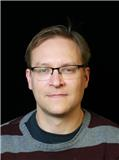
\includegraphics[width=.8\textwidth]{javier.jpeg} \\
Javier Gonz\'alez 
\end{minipage} ~
\begin{minipage}{0.3\textwidth}
\centering 
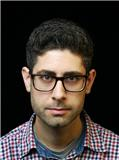
\includegraphics[width=.8\textwidth]{andreas.jpeg} \\
Andreas Damianou
\end{minipage} ~
\begin{minipage}{0.3\textwidth}
\centering 
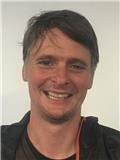
\includegraphics[width=.81\textwidth]{neil.jpeg} \\
Neil D. Lawrence
\end{minipage}

\end{frame}

% ====

\begin{frame}{Motivation}

\begin{itemize}
\item Bayesian Optimization aims at searching for the global minimum of an expensive function $g$,
\begin{equation*}\label{eq:min_problem}
\latentVector_{min} = \arg \min_{\latentVector \in {\mathcal X}} g(\latentVector).
\end{equation*}

\item What if the function $g$ is not directly measurable?
\end{itemize}
\end{frame}

\begin{frame}{Preference vs. Rating}

\begin{itemize}
\item The objective function of many tasks are difficult to precisely summarize into a single value.
\item Comparison is almost always easier than rating for humans.
\item Such observation has been exploited in A/B testing.
\end{itemize}
\centering
\vspace{-5mm}
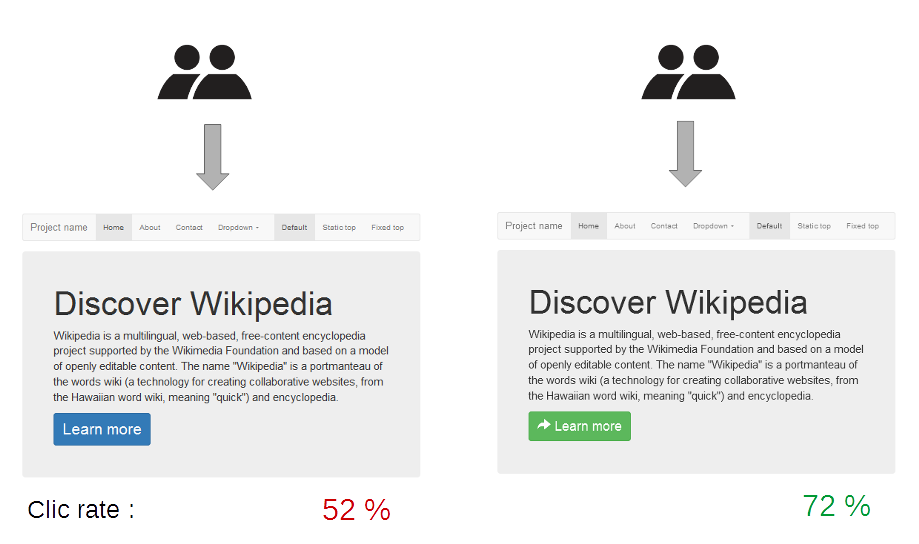
\includegraphics[width=0.6\textwidth]{A-B_testing_simple_example.png}
\end{frame}

\begin{frame}{BO via Preference}

\begin{itemize}
\item Beyond a single A/B testing.
\item To optimize a system via tuning this configuration, e.g., the font size, background color of a website.
\item The objective such as customer experience is not directly measurable
\item Compare the objective with two different configurations. 
\item The task is to search for the best configuration by iteratively suggesting pairs of configurations and observing the results of comparisons.
\end{itemize}
\centering
\vspace{-5mm}
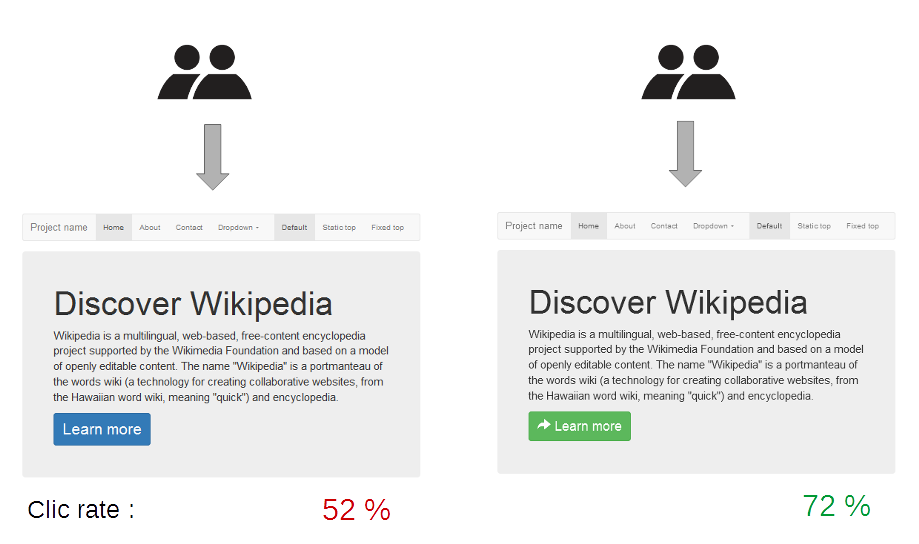
\includegraphics[width=0.6\textwidth]{A-B_testing_simple_example.png}
\end{frame}


\begin{frame}{Problem Definition}
\begin{itemize}
\item To find the minimum of a latent function $g(x), x \in {\mathcal X}$.
\item Observe only whether $g(\inputVector)<g(\inputVector')$ or not, for a \emph{duel} $[\inputVector,\inputVector'] \in {\mathcal X} \times {\mathcal X}$.
\item The outcomes are binary: \emph{true} or \emph{false}.
\item The outcomes are \emph{stochastic}.
\end{itemize}

\centering 
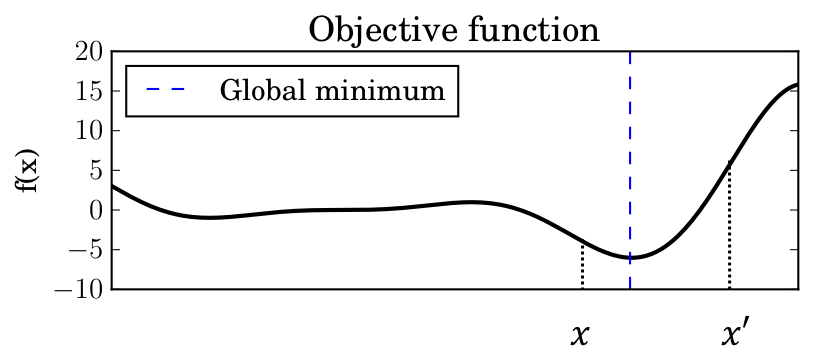
\includegraphics[width=.6\textwidth]{forrester_xx.png}
\end{frame}

\begin{frame}{Preference Function}
\begin{minipage}{0.5\textwidth}
\begin{itemize}
\item In this work, the probabilistic distribution is assumed to Bernoulli: \\
\begin{align*} &p(y \in \{0,1\} | [\inputVector,\inputVector'])= \pi^y(1-\pi)^{1-y},\\ 
&\pi = \sigma\Big(g(\inputVector') - g(\inputVector)\Big).
\end{align*}
\item $\pi$ is referred to as a \emph{preference function}.
\item A Preferential Bayesian optimization algorithm will propose a sequence of \emph{duels} that helps efficiently localize the minimum of a latent function $g( \inputVector)$.
\end{itemize}
\end{minipage}
~
\begin{minipage}{.45\textwidth}
\centering 

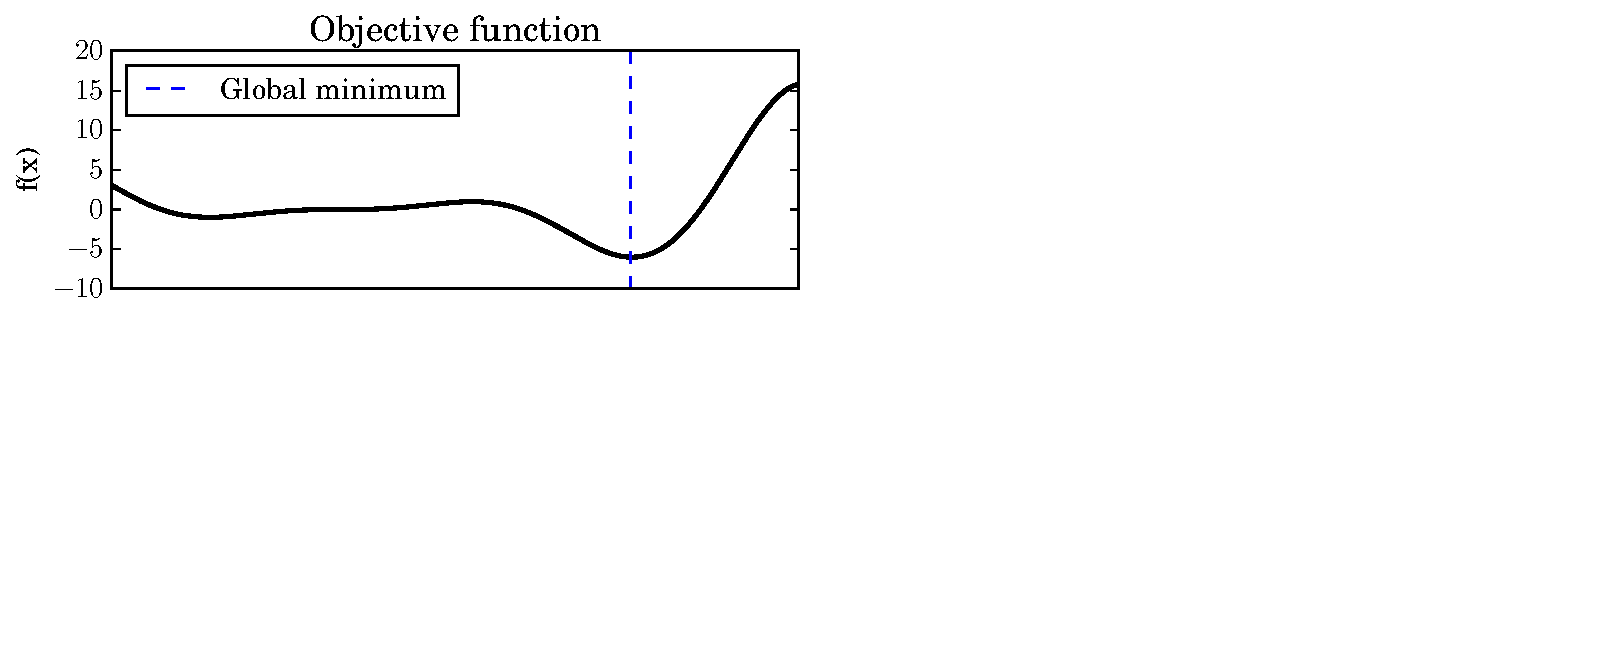
\includegraphics[width=.9\textwidth]{forrester.pdf}

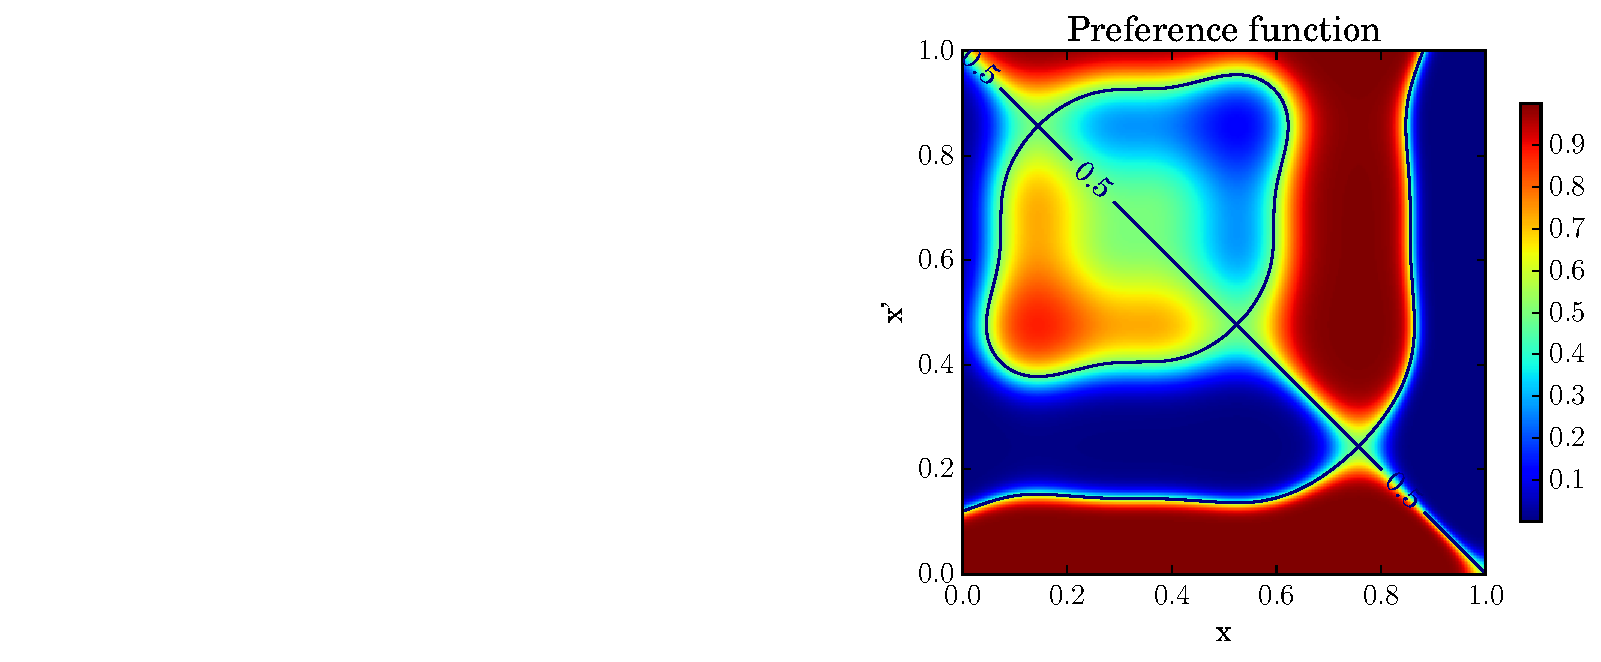
\includegraphics[width=.9\textwidth]{duel_space.pdf} 
\end{minipage}

\end{frame}

%\begin{frame}{A Concrete Example}
%\begin{minipage}{0.5\textwidth}
%\begin{itemize}
%\item 1D Forrester function:
%$$g(x) = (6x-2)^2\sin(12x-4)$$
%\item Leads to a 2D preference function $\pi$.
%\end{itemize}
%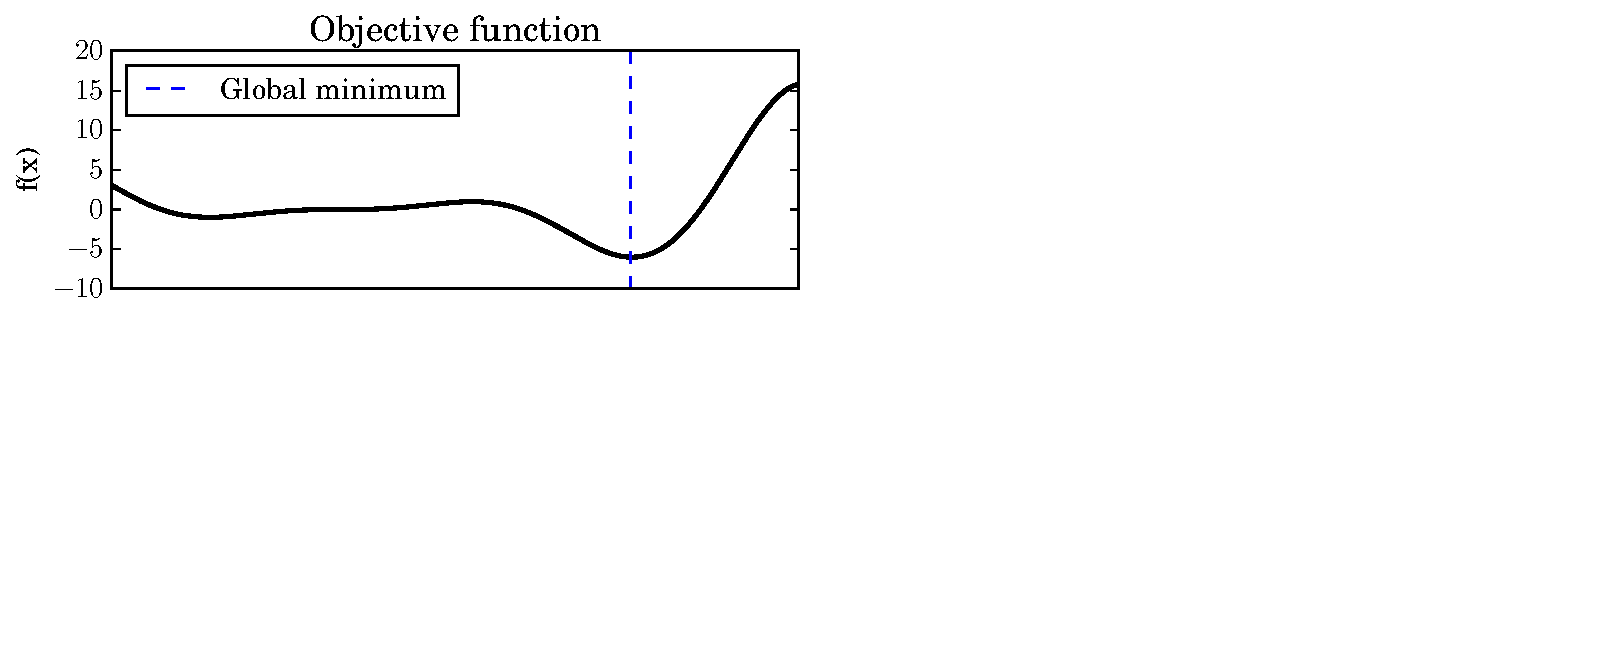
\includegraphics[width=1\textwidth]{forrester.pdf} 
%\end{minipage}
%~
%\begin{minipage}{.45\textwidth}
%\centering 
%
%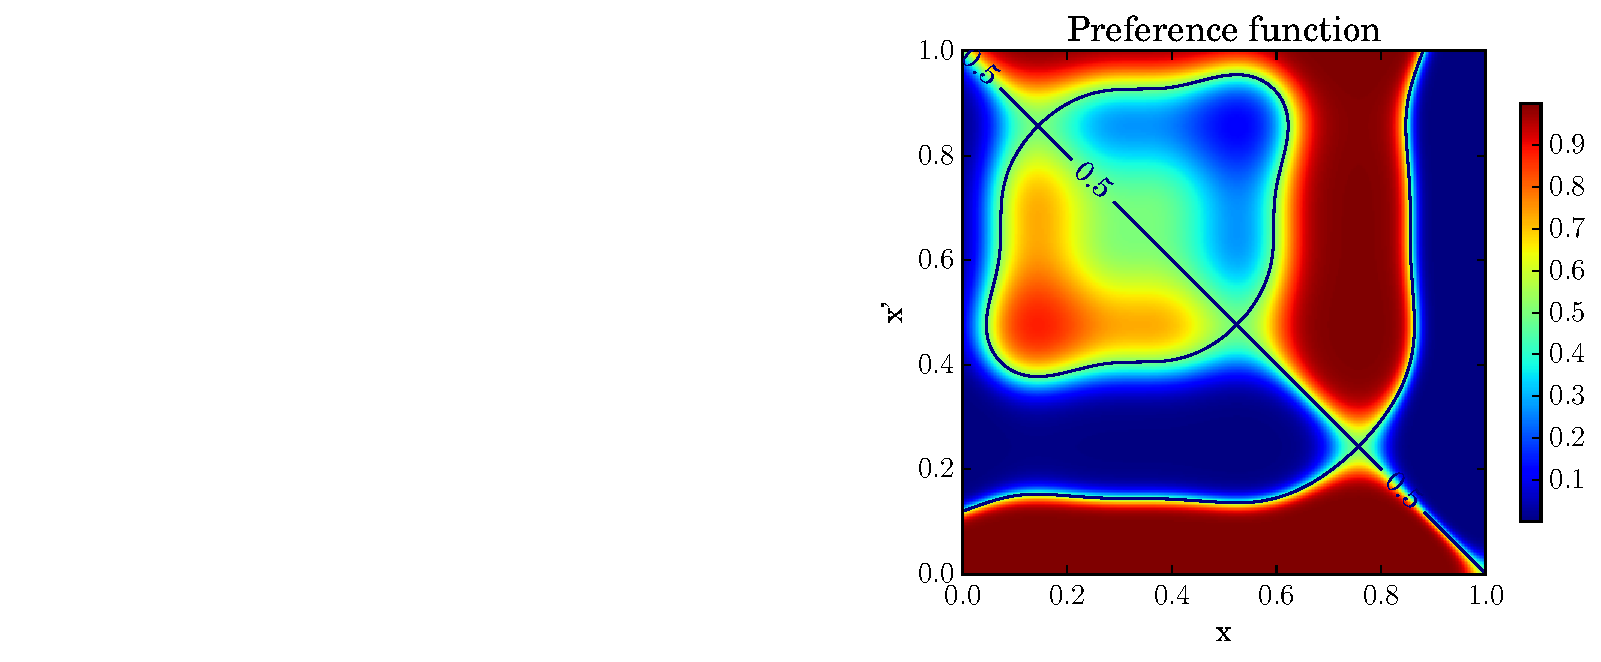
\includegraphics[width=1\textwidth]{duel_space.pdf} 
%\end{minipage}
%\end{frame}

\begin{frame}{A Surrogate Model}
\begin{minipage}{0.65\textwidth}

\begin{itemize}
%\item The evaluation of preference function requires the \emph{latent} function $g(\latentVector)$.
\item The preference function is not observable.
\item Only observe a few comparisons. 
\item Need a surrogate model to guide the search.
\item Two choices:
\begin{itemize}
\item  a surrogate model for the \emph{latent} function (like in standard BO). \citep{Brochu:2010, GuoEtAl2010}
\item a surrogate model for the preference function
 \end{itemize}
\end{itemize}
\end{minipage}
%
\begin{minipage}{0.33\textwidth}
\centering 
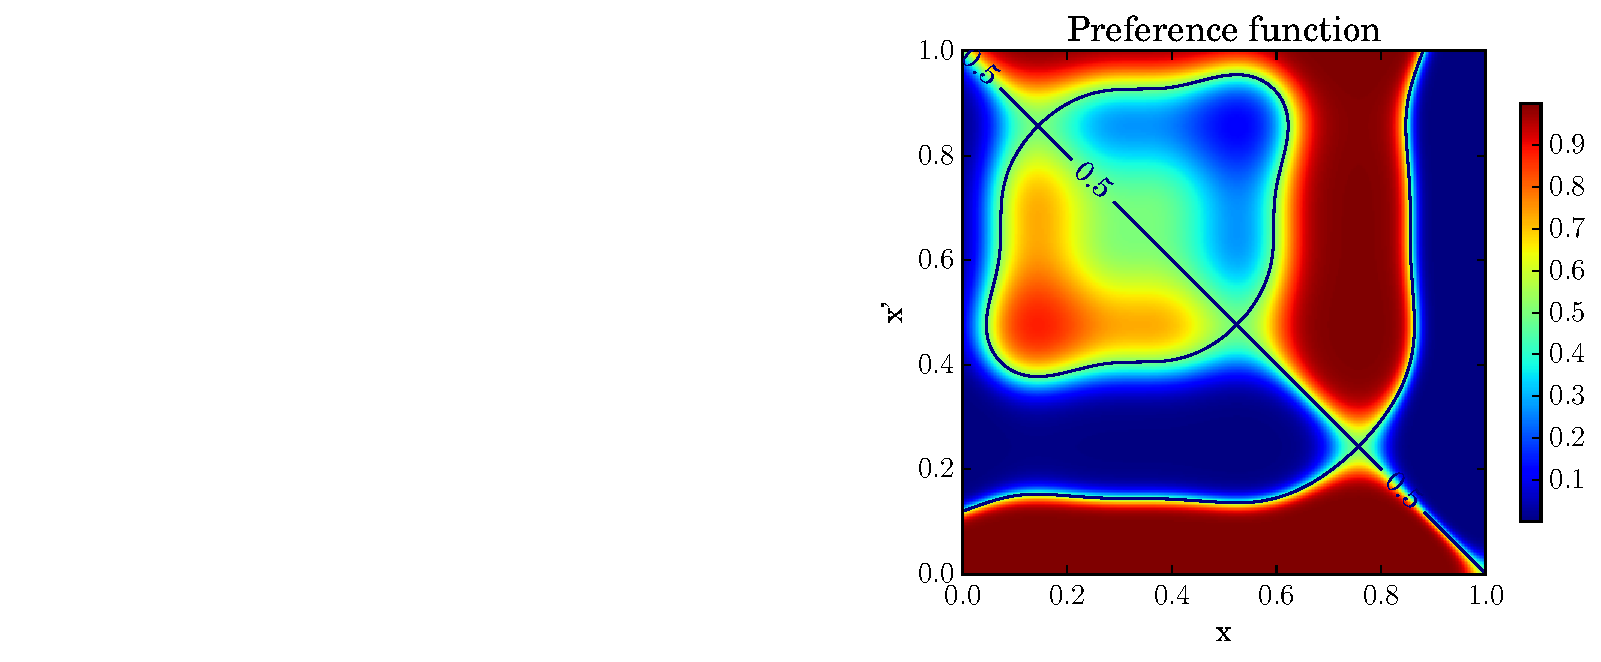
\includegraphics[width=1\textwidth]{duel_space.pdf} \\
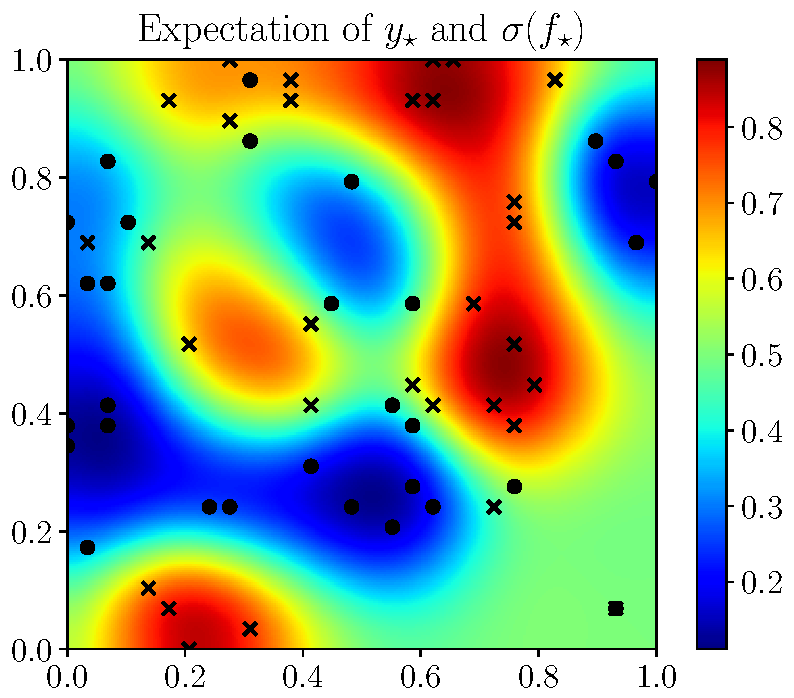
\includegraphics[width=.93\textwidth]{exp_y_star_cropped.pdf} 
\end{minipage}
\end{frame}

\begin{frame}{A Surrogate Model of Preference Model}
\begin{minipage}{0.65\textwidth}

\begin{itemize}
\item We propose to build a surrogate model for the preference function.
\item Pros: easy to model (Gaussian process Binary Classification is used:)
$$p(y_{\star} = 1 | \dataSet,  [\inputVector,\inputVector'], \theta) 
= \int \sigma(f_{\star}) p(f_{\star} | \dataSet, [\latentVector_{\star},\latentVector_{\star}'], \theta) df_{\star}$$
\item Pros: flexible latent function (e.g., non-stationality).
\item Cons: the minimum of the latent function is not directly accessible
\end{itemize}
\end{minipage}
%
\begin{minipage}{0.33\textwidth}
\centering 
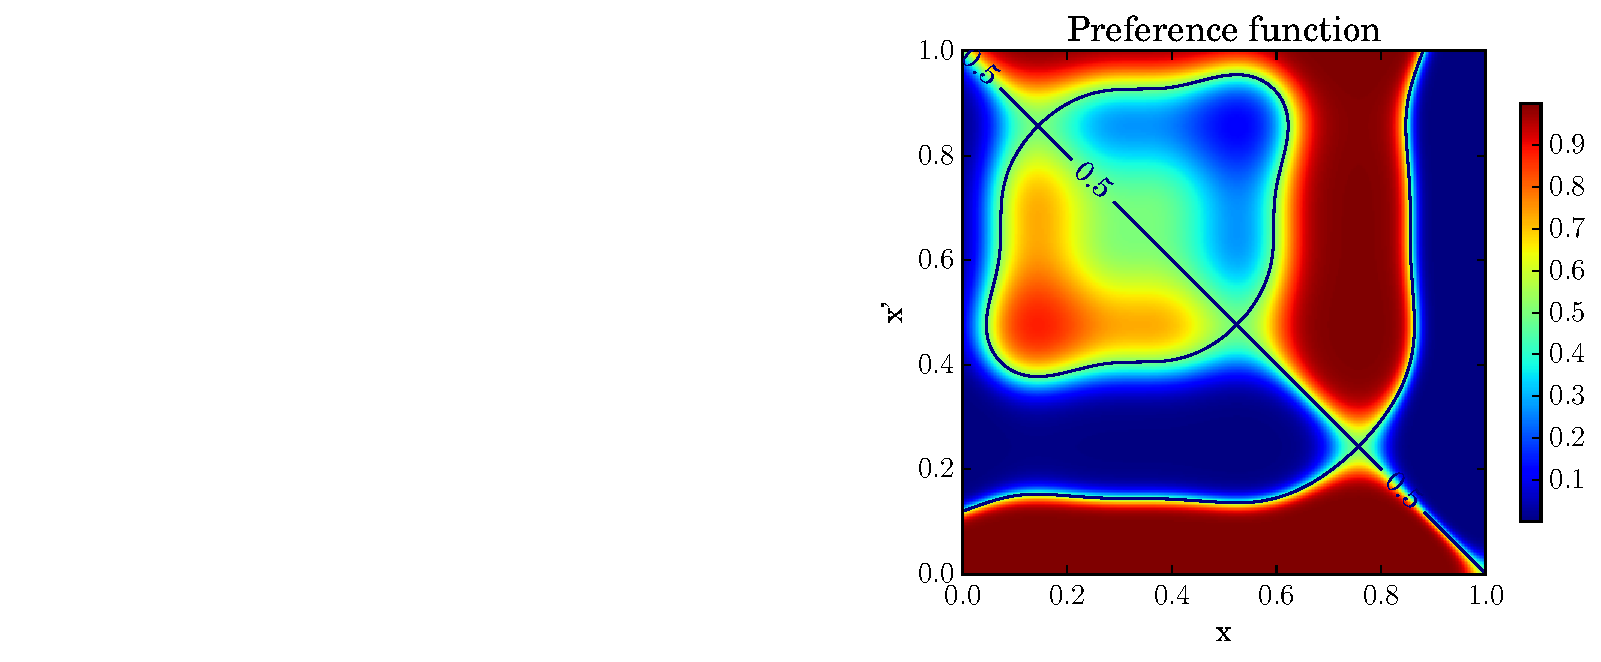
\includegraphics[width=1\textwidth]{duel_space.pdf} \\
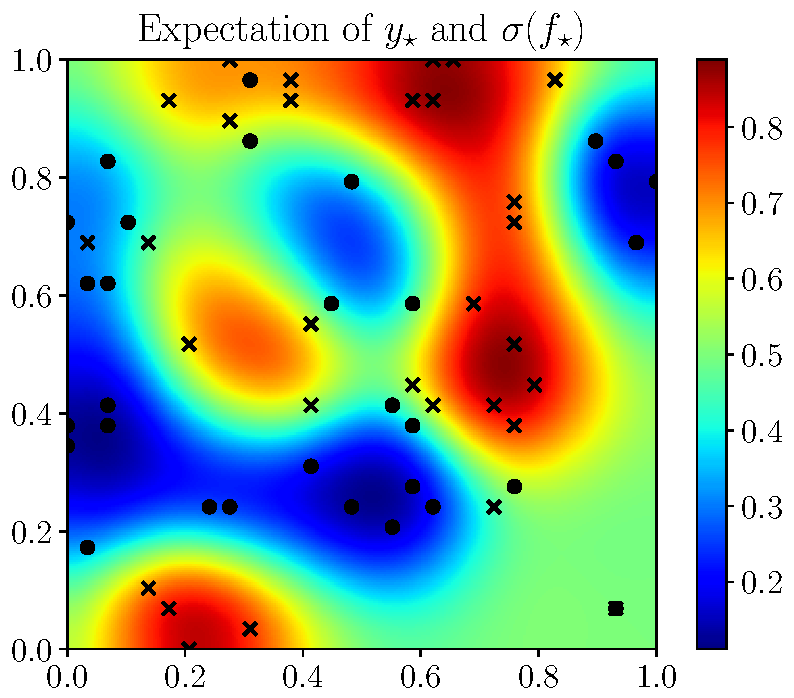
\includegraphics[width=.93\textwidth]{exp_y_star_cropped.pdf} 
\end{minipage}
\end{frame}

\begin{frame}{Who is the winner (the minimum)?}
\begin{itemize}
%\item \emph{normalised Copeland score}, already used in the literature of raking methods \citep{NIPS2015_6023} $S(\inputVector)= \text{Vol} ({\mathcal X})^{-1} \int_{\mathcal X} \mathbb{I}_{ \left\{\pi_{f}([\inputVector,\inputVector'])\geq0.5 \right\}} d\inputVector',$
\item The minimum beats \emph{all} the other locations on average.
\item Extending an idea from armed-bandits \citep{NIPS2015_6023}, we define the \emph{soft-Copeland} score as, (the average winning probability),
\begin{equation*}
C(\inputVector)= \text{Vol} ({\mathcal X})^{-1} \int_{\mathcal X} \pi_{f}([\inputVector,\inputVector']) d\inputVector',
\end{equation*}
\item The optimum of $g(\inputVector)$ can be estimated as, denoted as the \emph{Condorcet} winner,
$$x_{c} = \arg \max_{\latentVector \in {\mathcal X}} C(\latentVector),$$
\end{itemize}
%
\centering
\vspace{-5mm}
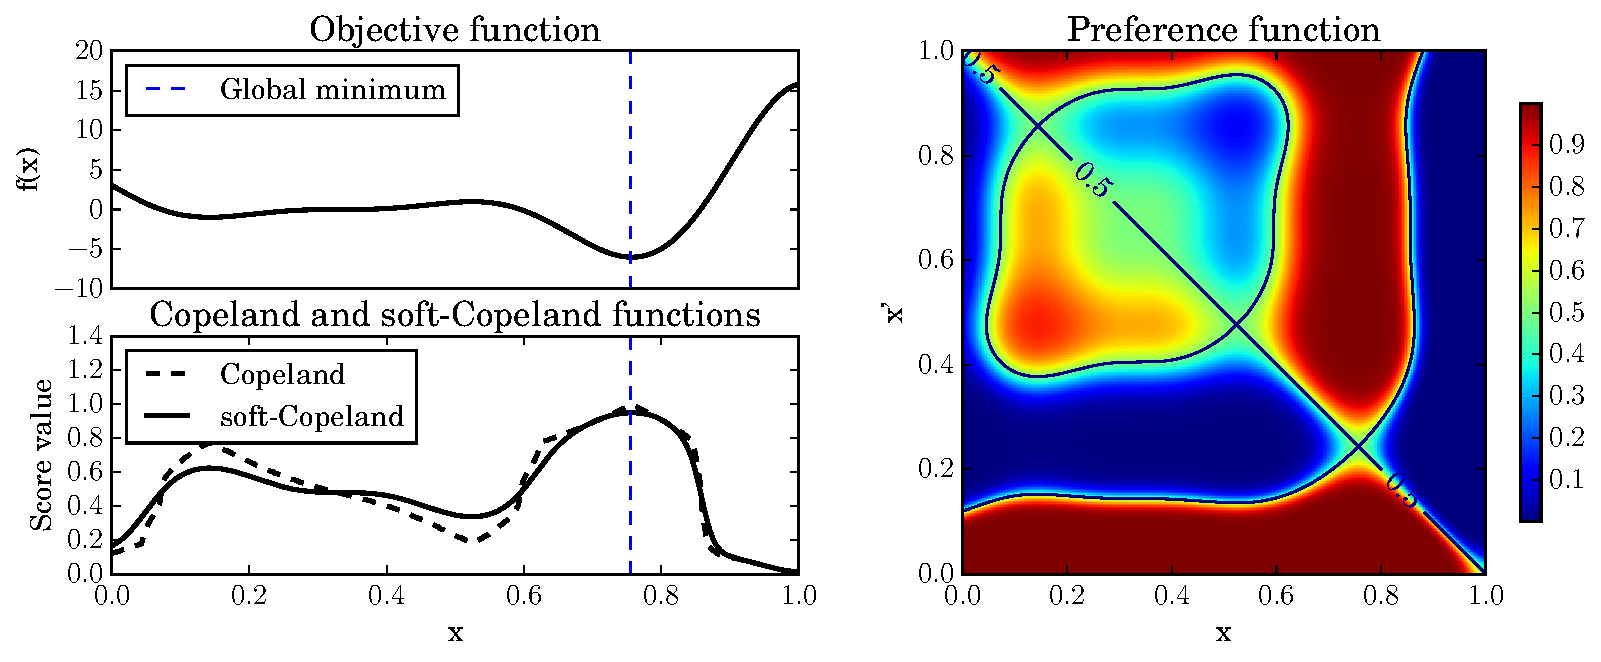
\includegraphics[width=0.75\textwidth]{condorcet.pdf}
\end{frame}

\begin{frame}{The current estimation of minimum}
\begin{itemize}
\item Only have a surrogate model of preference function.
\item Estimate the \emph{soft-Copeland} score from the surrogate model and get an approximate \emph{Condorcet} winner.
\item Note that the approximated \emph{Condorcet} winner may \emph{not} be the optimum of $g(\inputVector)$.
\end{itemize}
%
%\centering
%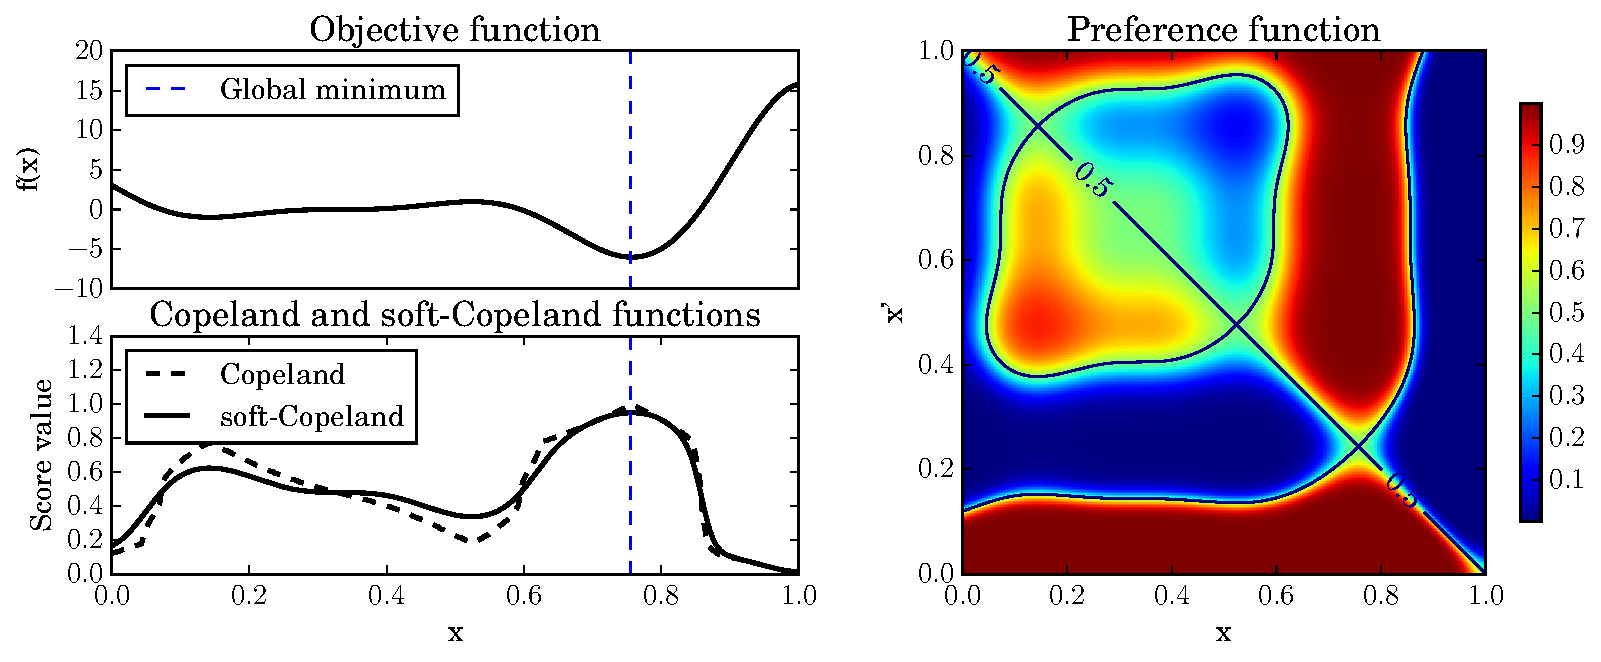
\includegraphics[width=0.75\textwidth]{condorcet.pdf}
\end{frame}


\begin{frame}{Acquisition Function}
\begin{minipage}{0.65\textwidth}
\begin{itemize}
\item Existing Acq. Func. are not \emph{applicable}.
\item They are designed to work with a surrogate model of the objective function.
\item In PBO, the surrogate model does not directly represent the \emph{latent} objective function.
\item We need a new Acq. Func. for duels!
\end{itemize}
\end{minipage}
%
\begin{minipage}{0.33\textwidth}
\centering 
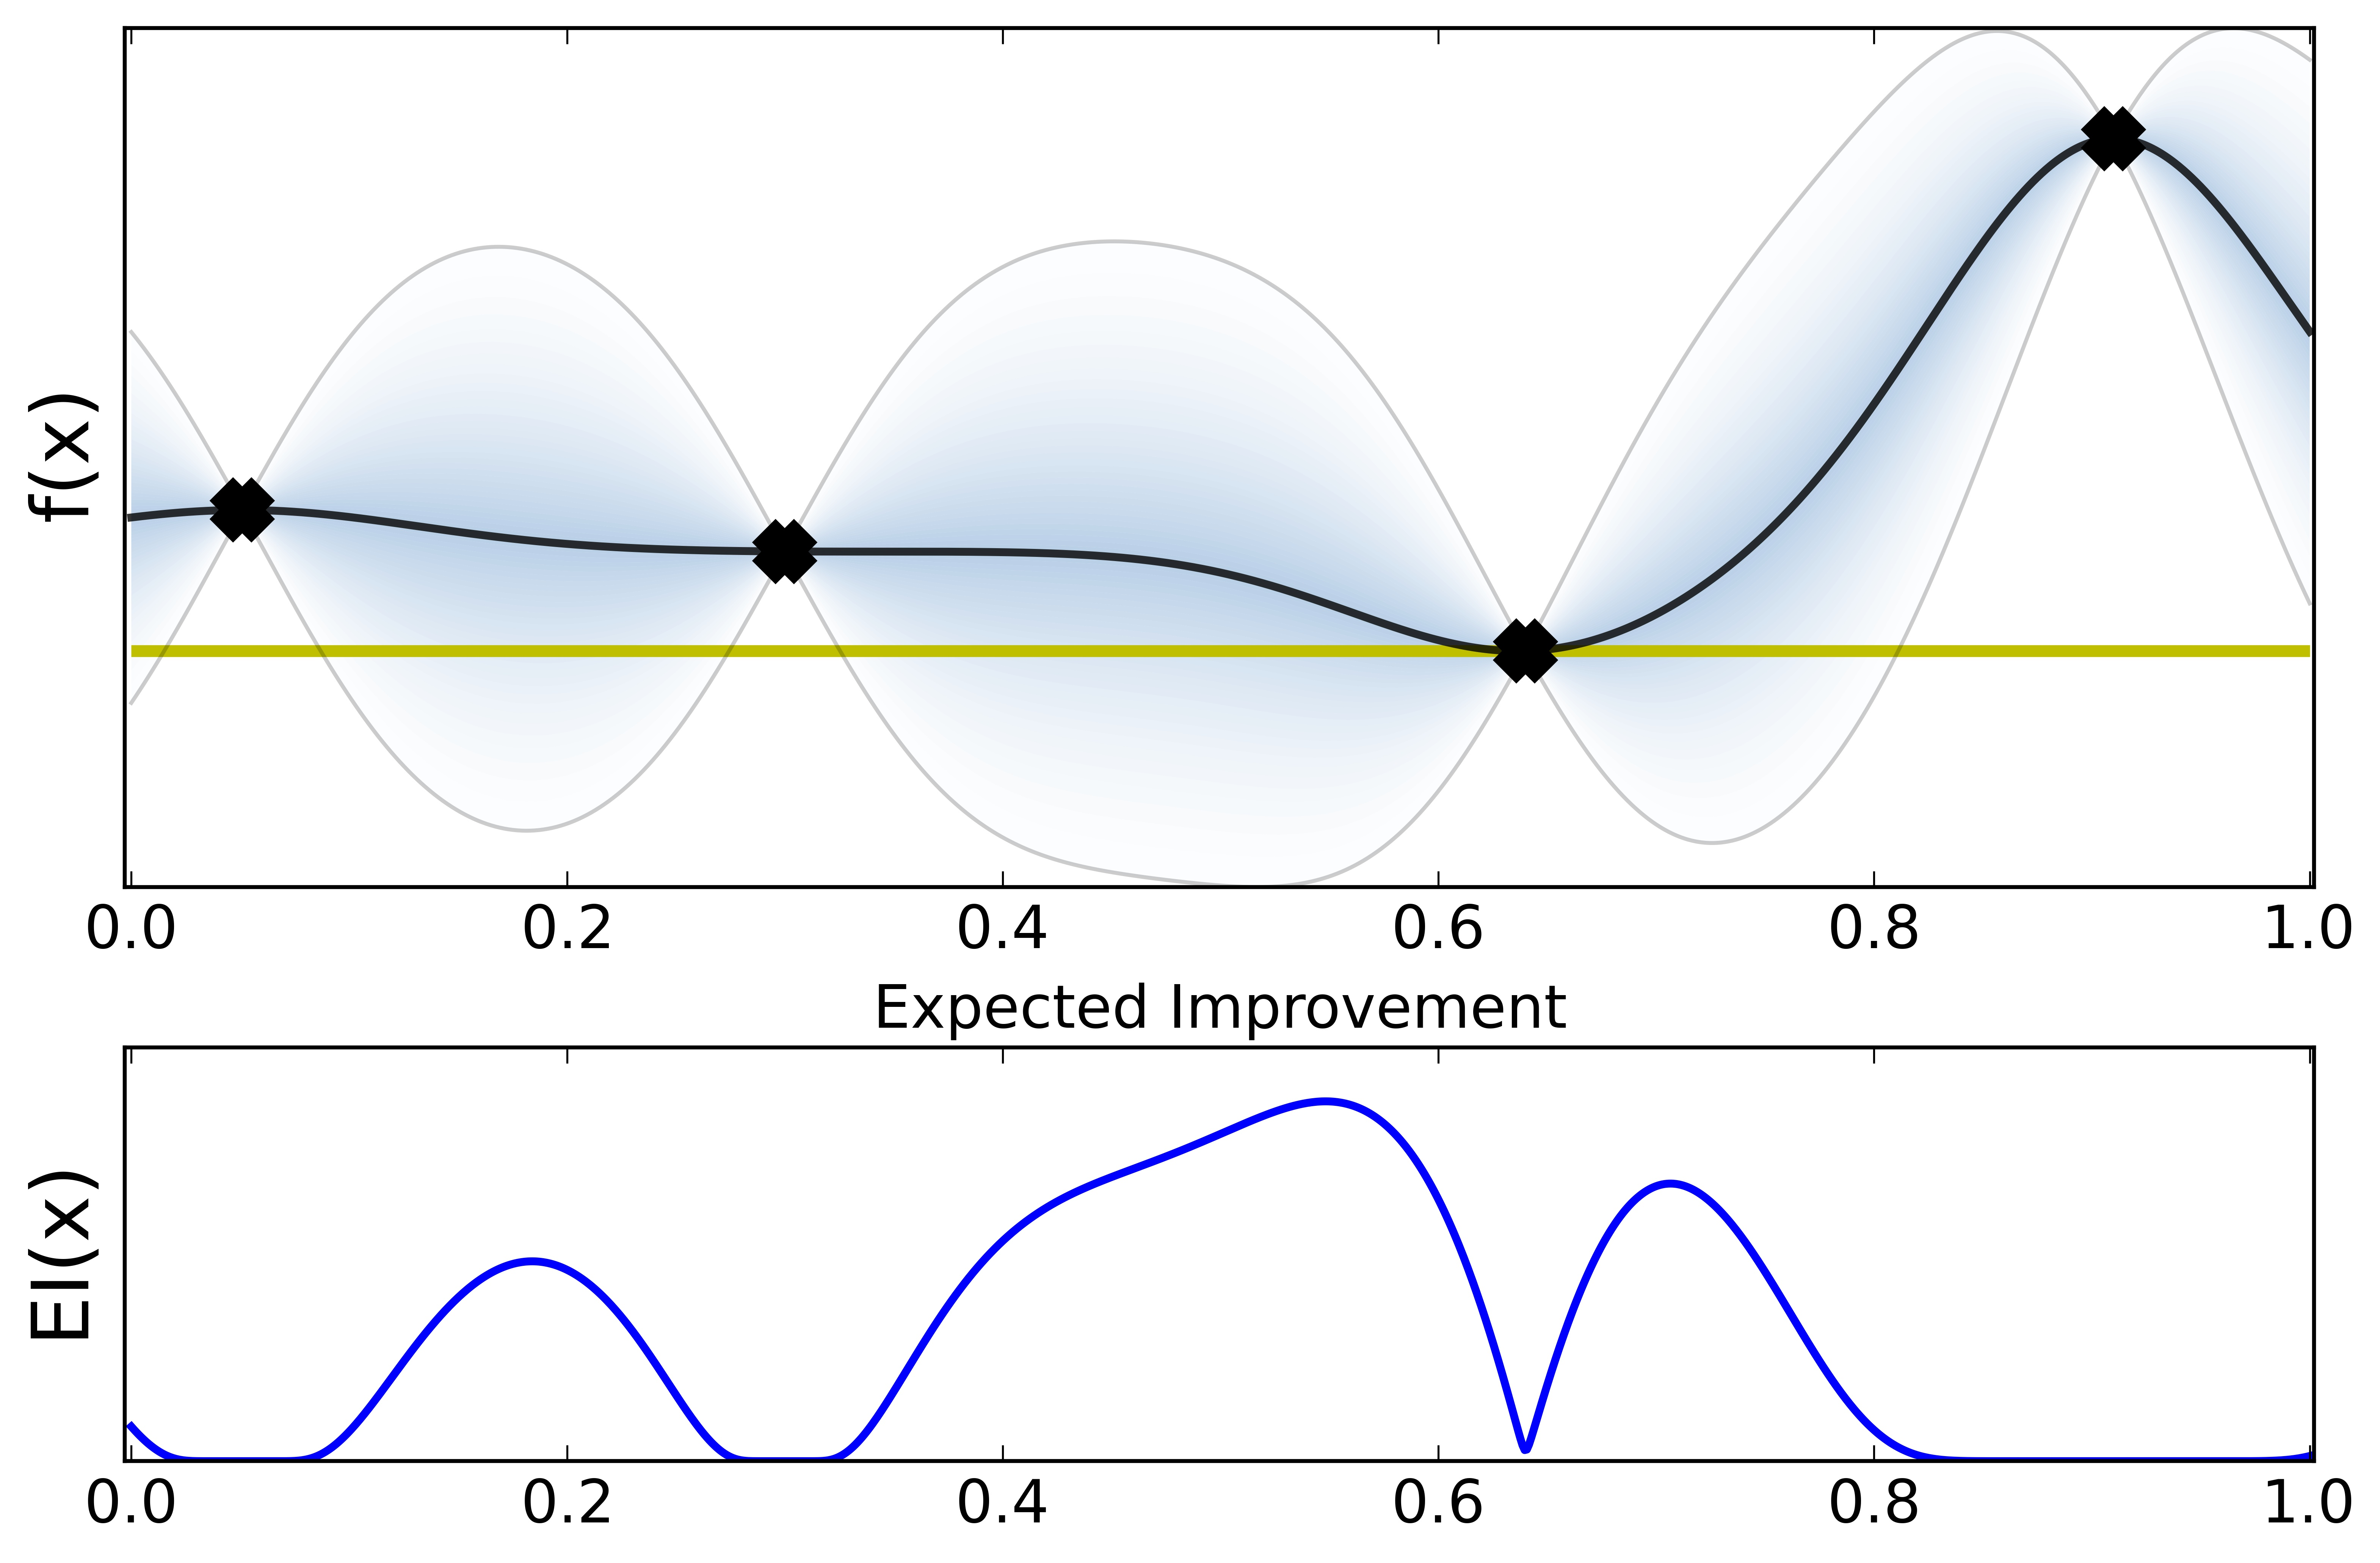
\includegraphics[width=1\textwidth]{EI.jpeg} \\
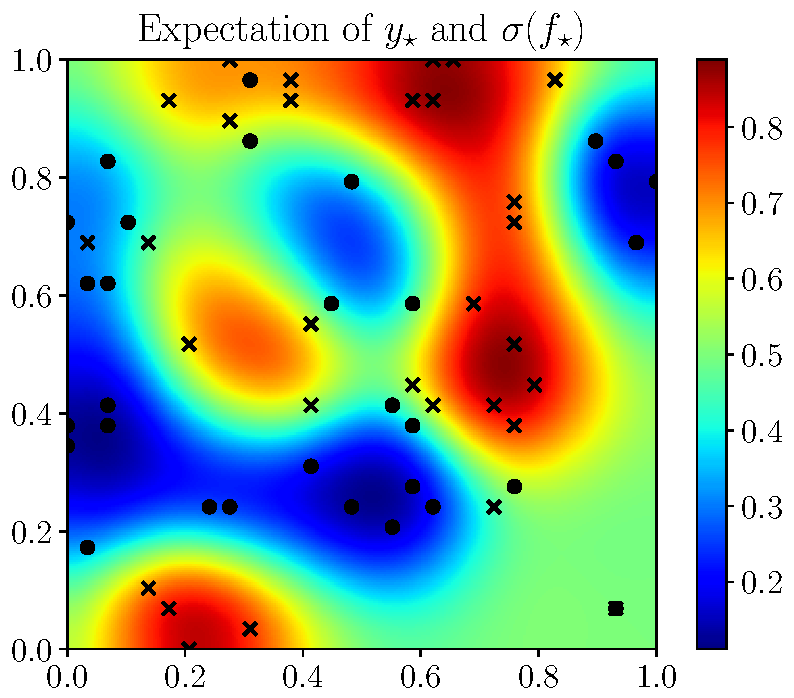
\includegraphics[width=.93\textwidth]{exp_y_star_cropped.pdf} 
\end{minipage}
\end{frame}

\begin{frame}{Pure Exploration Acquisition Function (PBO-PE)}
\begin{minipage}{0.65\textwidth}
\begin{itemize}
\item The common pure explorative acq. func., \emph{i.e.} $\V[y]$, does not work.
\item Propose a pure explorative acq. func. as the variance (uncertainty) of the ``winning" probability of a duel:
$$
\V[ \sigma(f_{\star})]  = \int \left(\sigma(f_{\star}) - \E[ \sigma(f_{\star})] \right)^2 p (f_{\star} | \dataSet,  [\inputVector,\inputVector']) df_{\star} 
$$
\end{itemize}
\end{minipage}
%
\begin{minipage}{0.33\textwidth}
\centering 
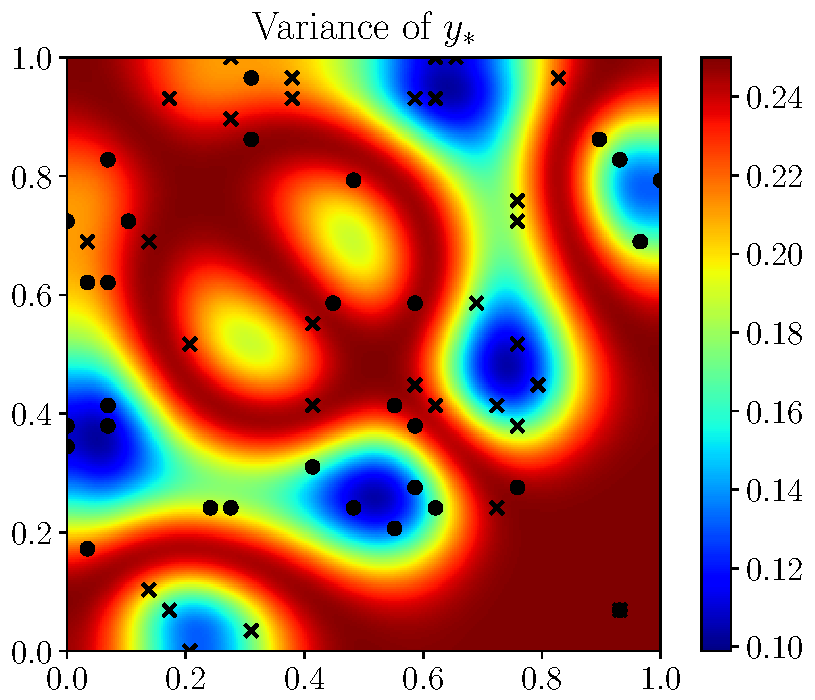
\includegraphics[width=0.95\textwidth]{var_y_star_cropped.pdf} \\
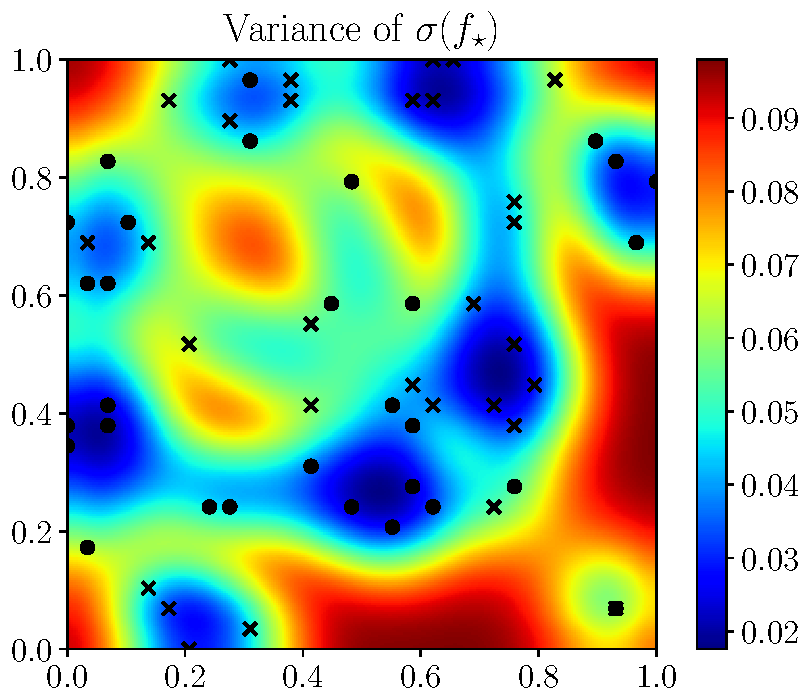
\includegraphics[width=0.95\textwidth]{var_f_star_cropped.pdf}
\end{minipage}
\end{frame}



\begin{frame}{Acquisition Function: PBO-DTS}
To select the next duel $[\inputVector_{next}, \inputVector_{next}']$:
\begin{enumerate}
\item Draw a sample from surrogate model
\item Take the maximum of \emph{soft-Copeland} score as $\inputVector_{next}$.
\item Take $\inputVector_{next}'$ that gives the maximum in PBO-PE
\end{enumerate}

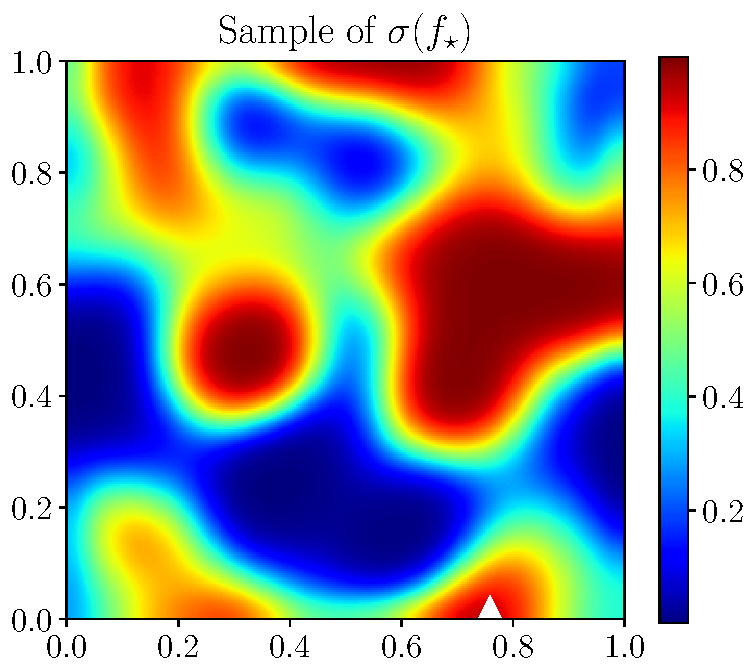
\includegraphics[width=0.335\textwidth]{sample_f_star_cropped.pdf} 
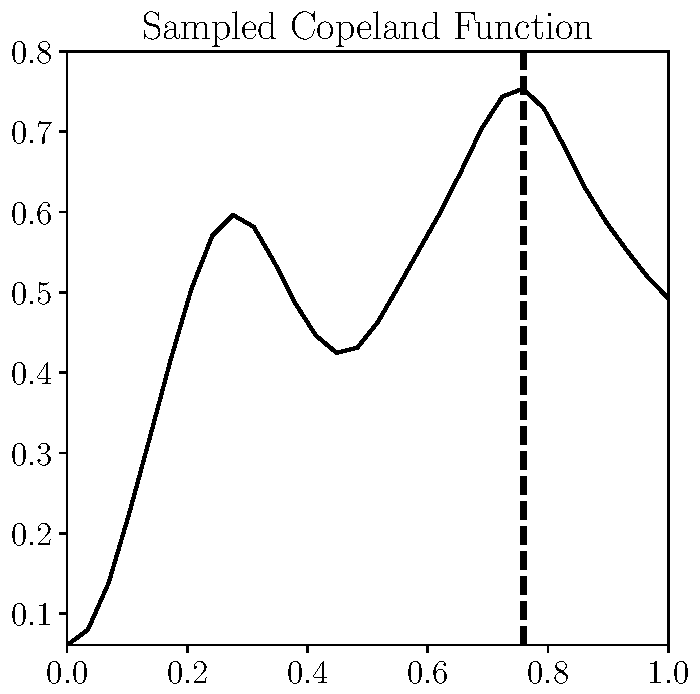
\includegraphics[width=0.295\textwidth]{sample_copeland_cropped.pdf} 
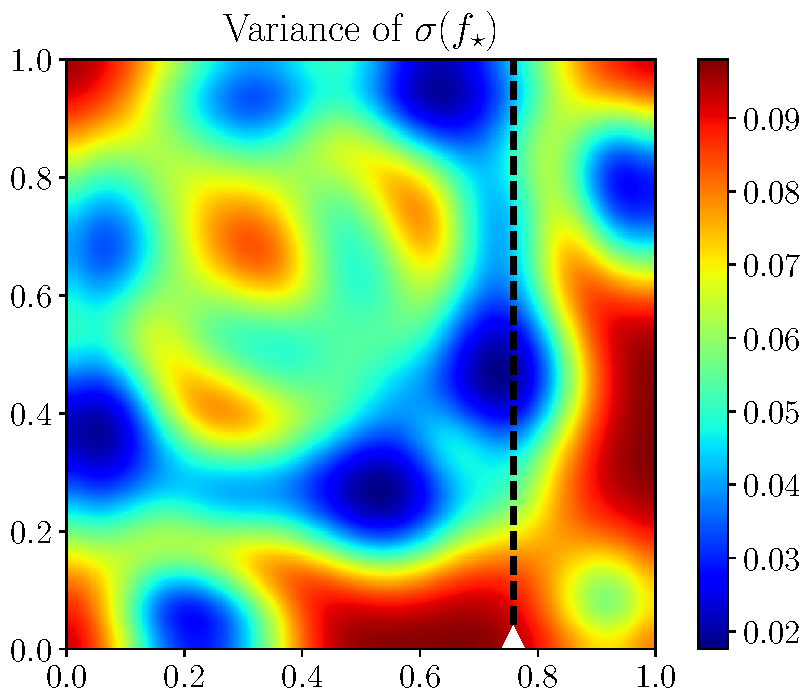
\includegraphics[width=0.34\textwidth]{var_f_max_cropped.pdf} 

%Illustration of the steps to propose a new duel using the duelling-Thompson acquisition. The duel is computed using the same model as in Figure \ref{fig:exploration}. The white triangle represents the final selected duel. \emph{Left:} Sample from $f_{\star}$ squashed through the logistic function $\sigma$. \emph{Center:} Sampled soft-Copeland function, which results from integrating the the sample from $\sigma(f_{\star})$ on the left across the vertical axis. The first element of the duel $\inputVector$ is selected as the location of the maximum of the sampled soft-Copeland function (vertical dotted line). \emph{Right:} The second element of the duel, $\inputVector'$, is selected by maximizing the variance of $\sigma(f_{\star})$ marginally given $\inputVector$ (maximum across the vertical dotted line).
\end{frame}

\begin{frame}{Experiment: Forrester Function}
\begin{minipage}{0.36\textwidth}
\begin{itemize}
\item Synthetic 1D function: Forrester
\item Observations drawn with a probability: 
$ \frac1{1+e^{g(\latentVector)-g(\latentVector')}}$
\item $g(x_c)$ shows the value at the location that algorithms \emph{believe} is the minimum.
\item The curve is the average of 20 trials.
\end{itemize}

\begin{flushleft}
\tiny
IBO: \citep{Brochu:2010}\\
SPARRING: \citep{AilonKJ14}
\end{flushleft}
\end{minipage}
%
\begin{minipage}{.63\textwidth}
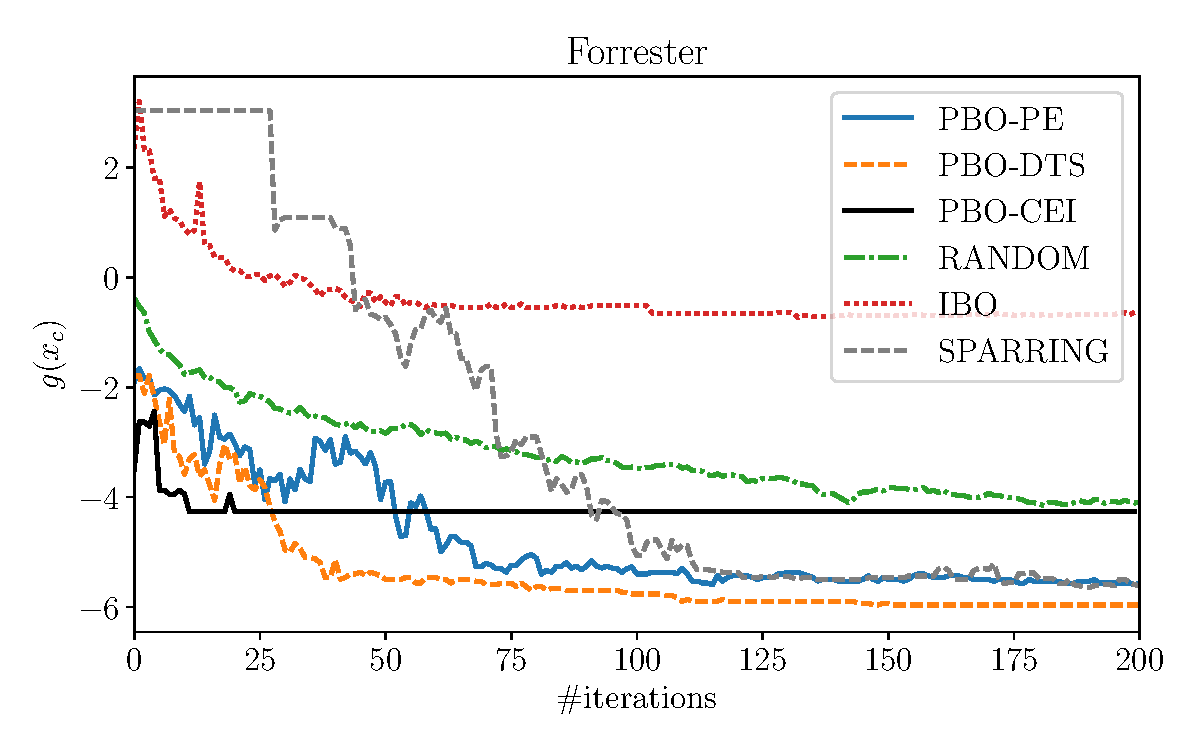
\includegraphics[width=1.\textwidth]{results_forrester_new.pdf}
\end{minipage}
\end{frame}

\begin{frame}{Experiments: More (2D) Functions}
\begin{center}
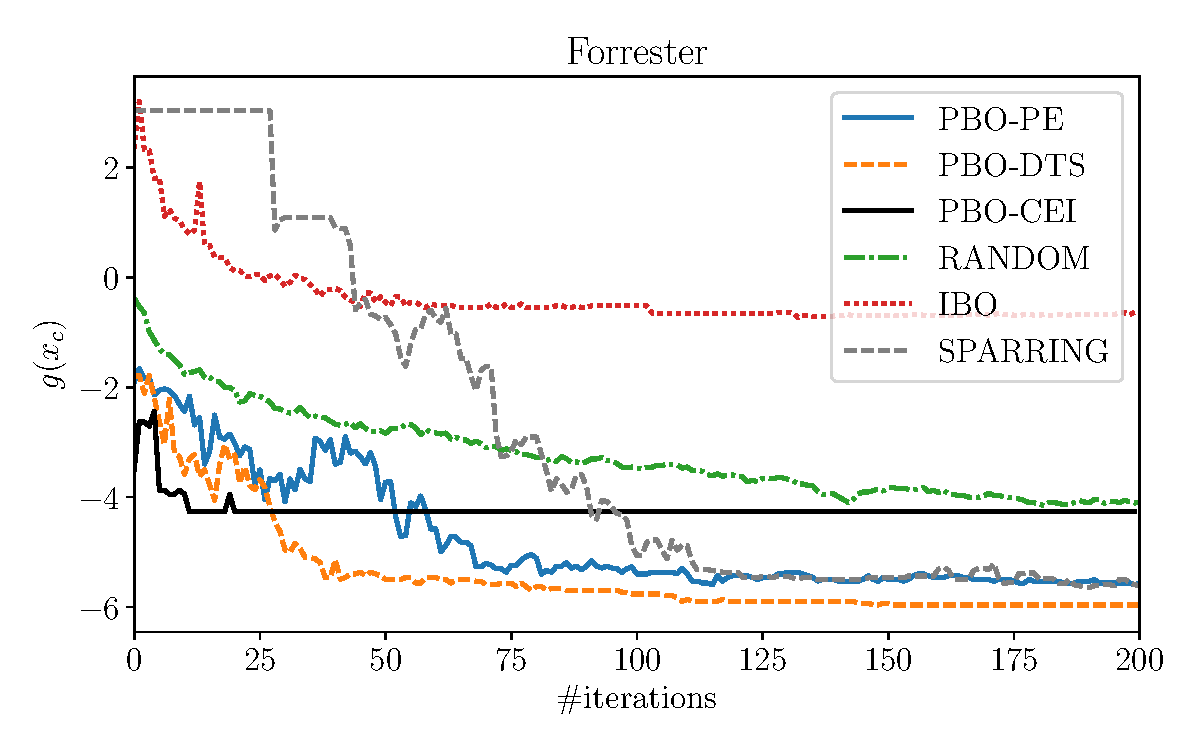
\includegraphics[width=0.45\textwidth]{results_forrester_new.pdf} ~
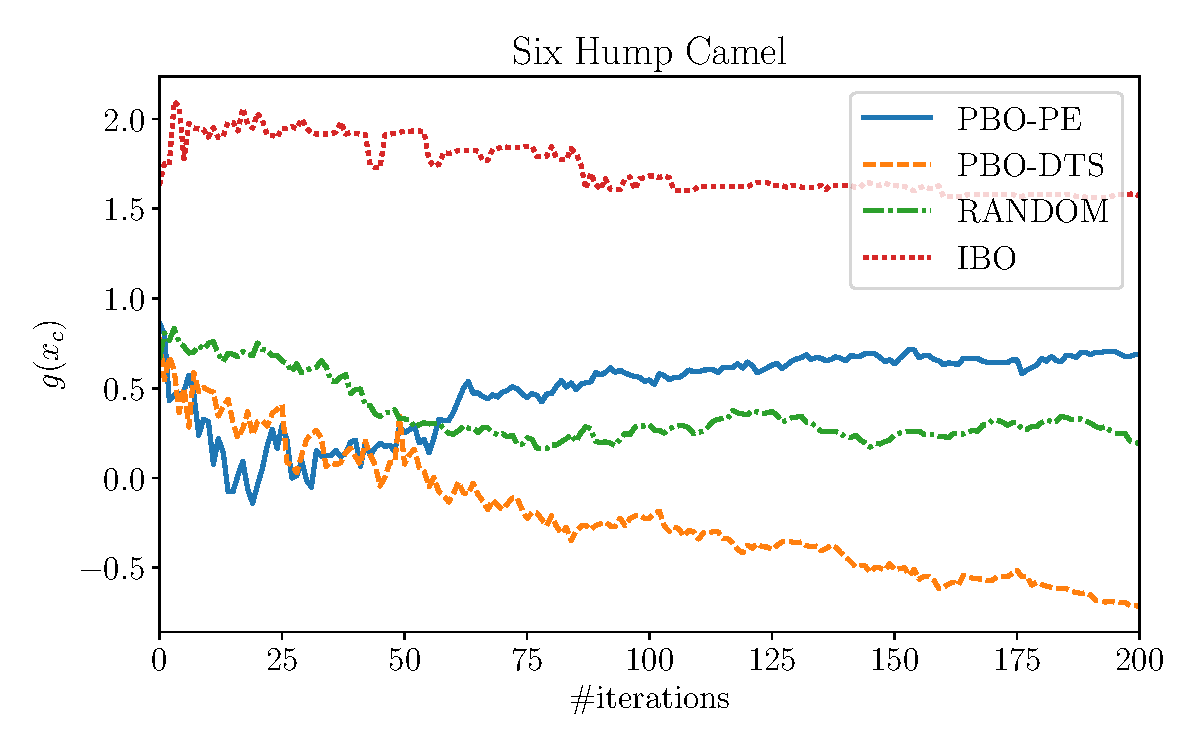
\includegraphics[width=0.45\textwidth]{results_sixhump_new.pdf} \\
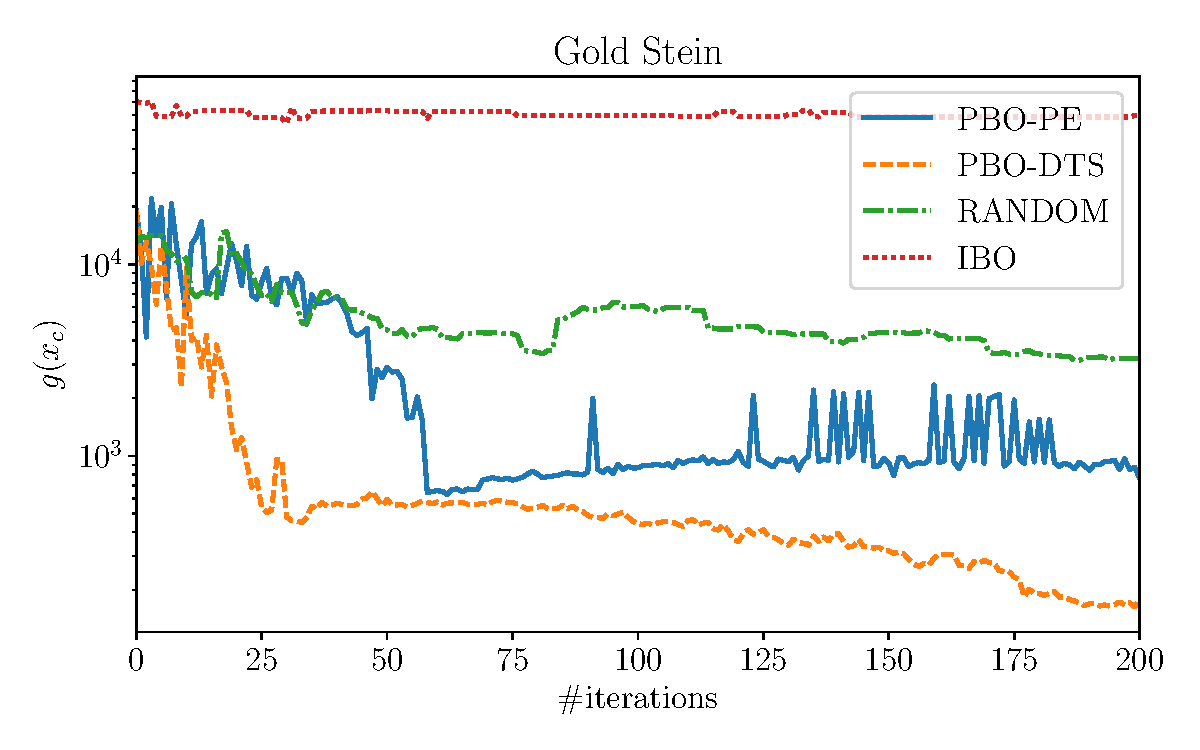
\includegraphics[width=0.45\textwidth]{results_goldstein.pdf} ~
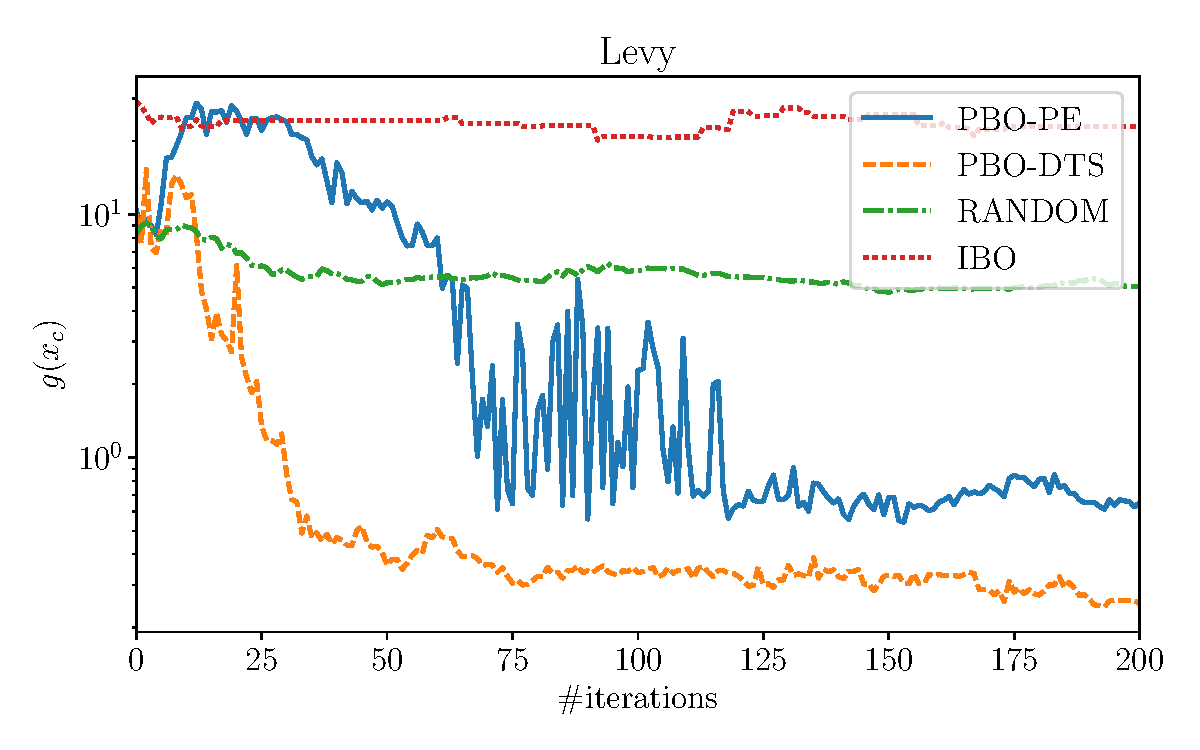
\includegraphics[width=0.45\textwidth]{results_levy.pdf} 
\end{center}
\end{frame}

\begin{frame}{Summary}
\begin{itemize}
\item Address Bayesian optimization with preferential returns.
\item Propose to build a surrogate model for the preference function.
\item Propose a few efficient acquisition functions.
\item Show the performance on synthetic functions.
\end{itemize}
\end{frame}

\begin{frame}{}
Questions?
\end{frame}


% ====
\appendix

\begin{frame}{Exploration \& Exploitation}
\centering
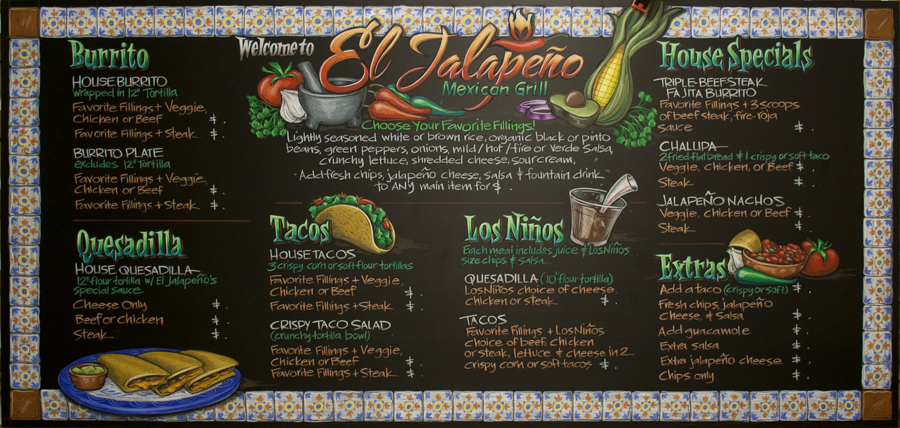
\includegraphics[width=.93\textwidth]{menu.jpg} 

The two ingredients in an acquisition function: Exploration \& Exploitation.
\end{frame}

\begin{frame}{Exploration in PBO}
\begin{minipage}{0.65\textwidth}
\begin{itemize}
\item To understand exploration in PBO by designing a \emph{pure explorative} acq. func.
\item Exploration in standard BO can be viewed as the action to reduce uncertainty of a surrogate model.
\item A purely explorative acq. func. 
$$\V[ y_{\star}]  = \int \left(y_{\star} - \E[ y_{\star}] \right)^2 p (y_{\star} | \dataSet,  \inputVector_\star) \dif{y_{\star}} $$
\item Can we extend this idea to PBO?
\end{itemize}
\end{minipage}
%
\begin{minipage}{0.33\textwidth}
\centering 
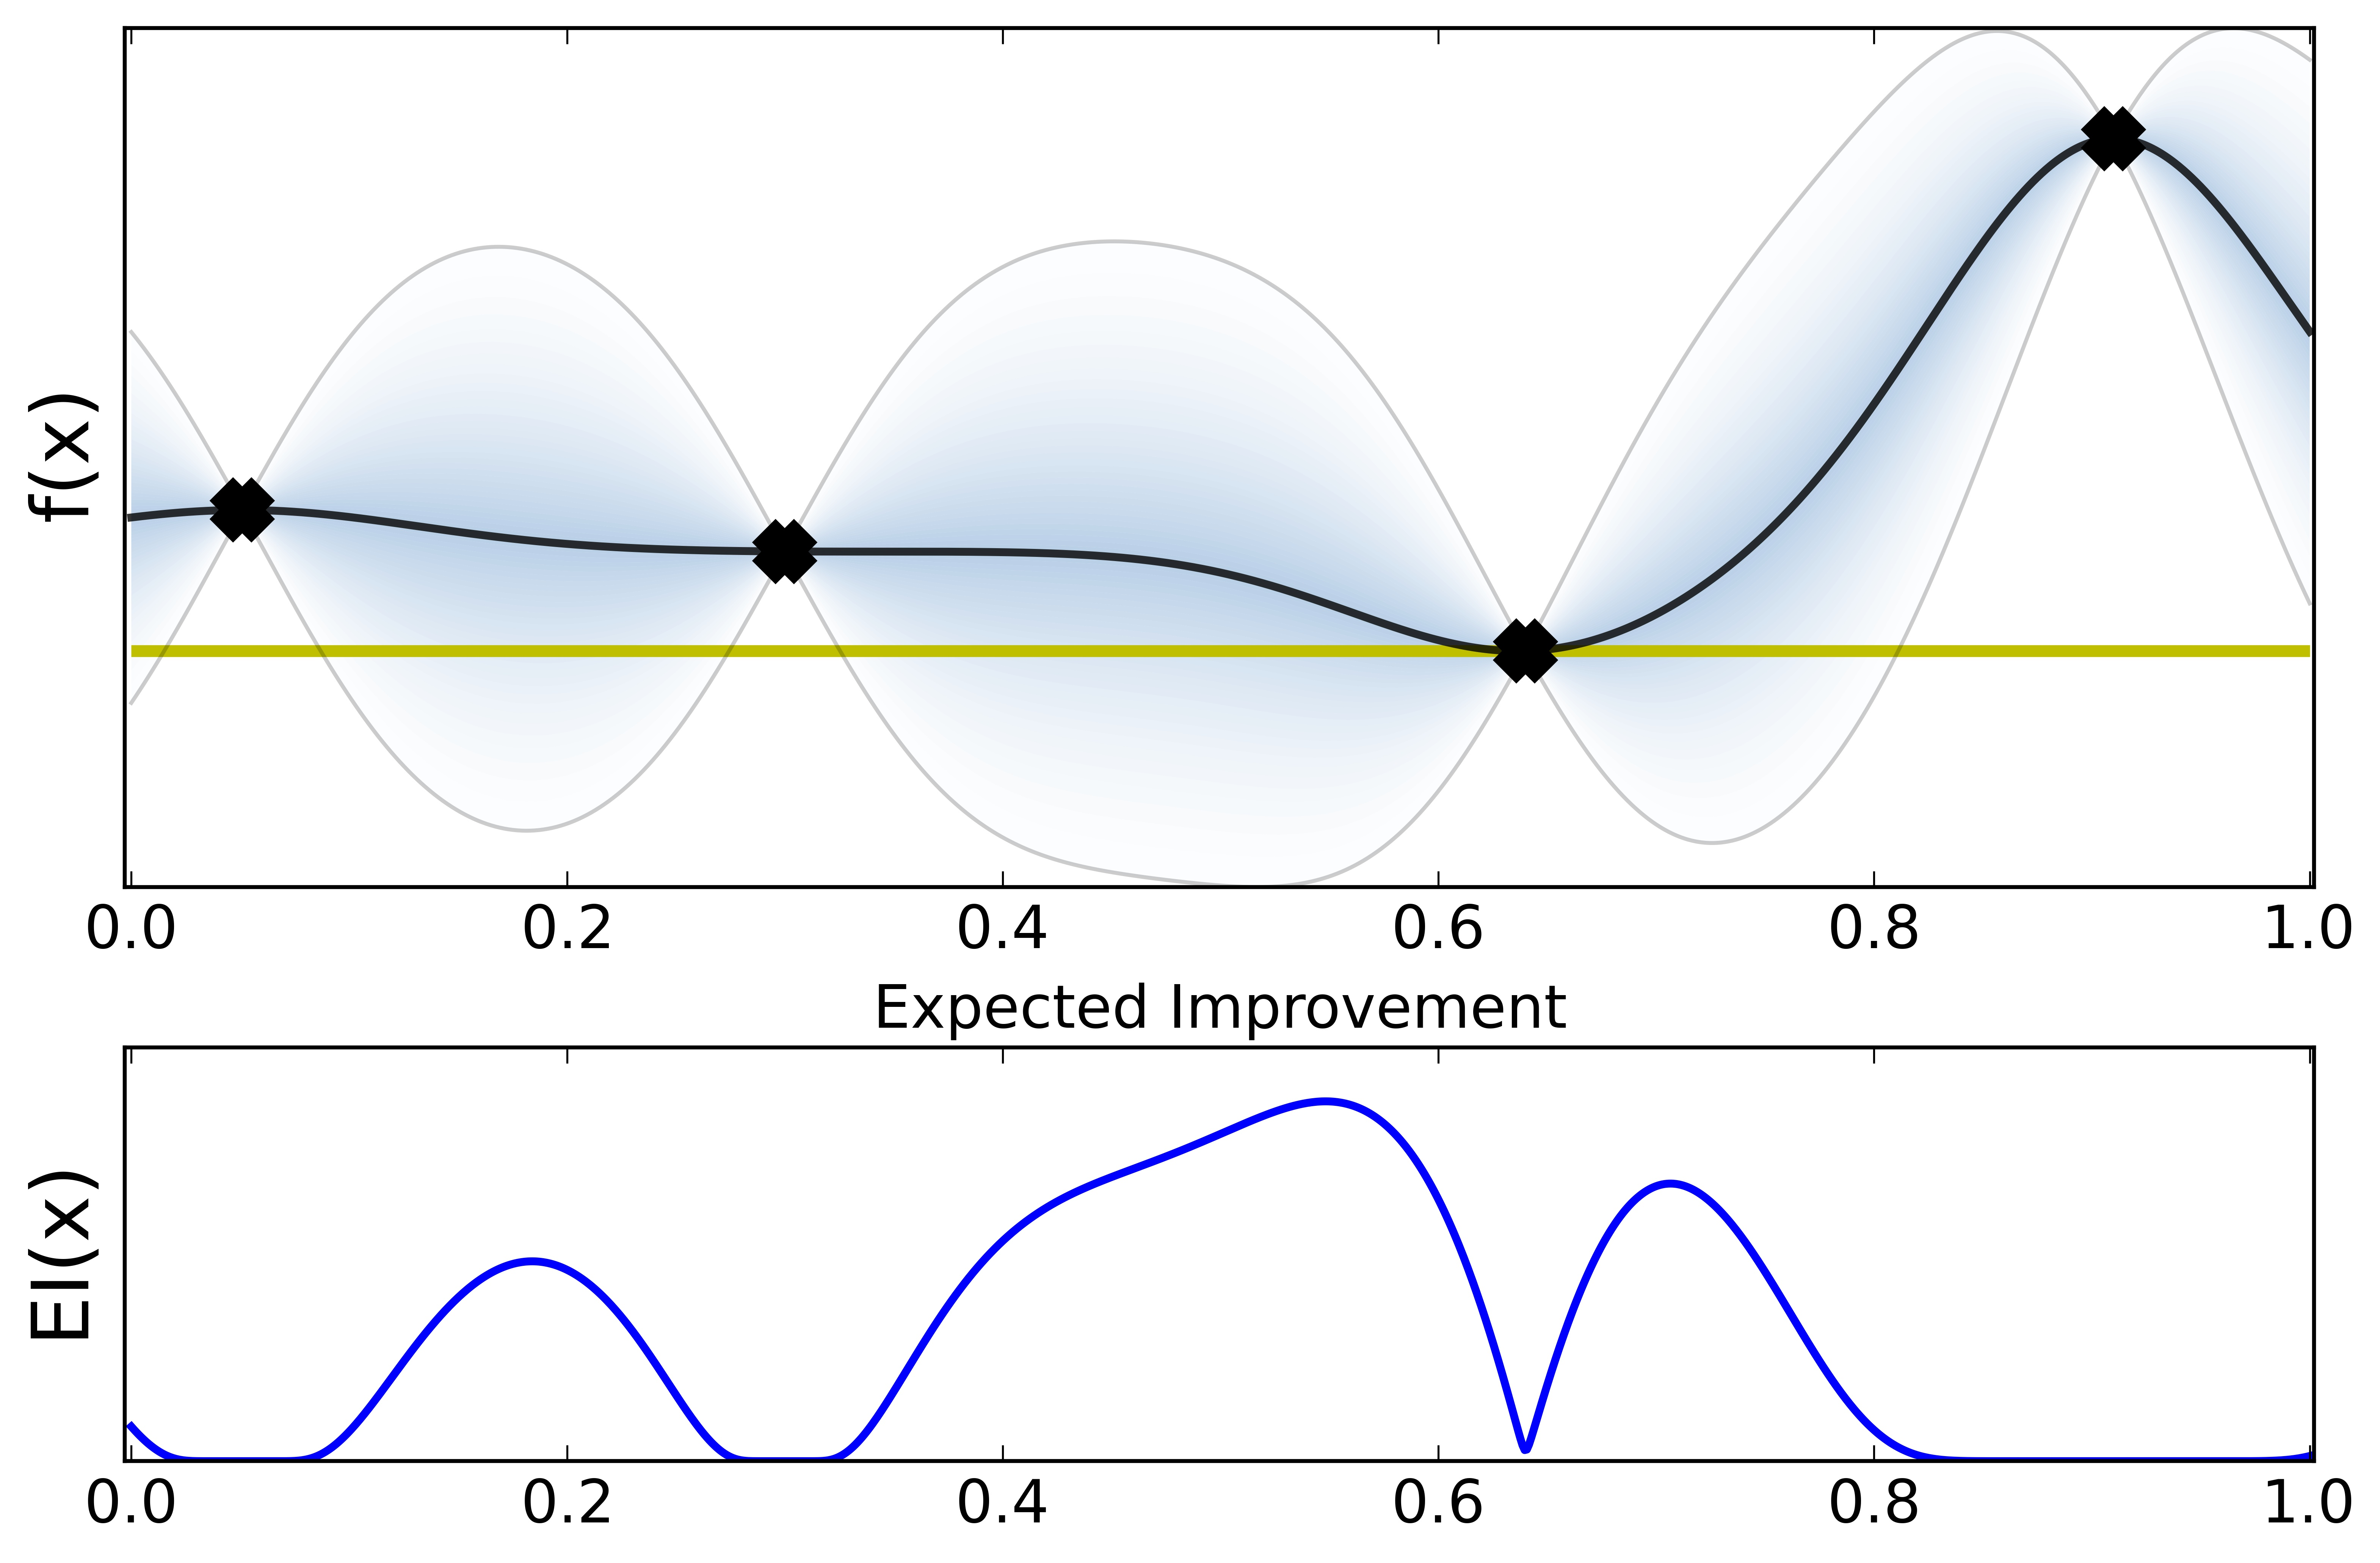
\includegraphics[width=1.\textwidth]{EI.jpeg}
\end{minipage}
\end{frame}

\begin{frame}{A Straight-Forward Choice}
\begin{minipage}{0.65\textwidth}
\begin{itemize}
\item A straight-forward extension from standard BO:
\begin{align*}
\V[ y_{\star}]  =& \sum_{y_{\star}\in\{0,1\}} \left(y_{\star} - \E[ y_{\star}] \right)^2 p (y_{\star} | \dataSet,  [\inputVector_\star,\inputVector_\star'])\\
=& \E[ y_{\star}](1-\E[ y_{\star}])
\end{align*}
\item The maximum variance is always at where $\E[ y_{\star}]=0.5$!
\item The variance may not reduce with observations!
\end{itemize}
\end{minipage}
%
\begin{minipage}{0.33\textwidth}
\centering 
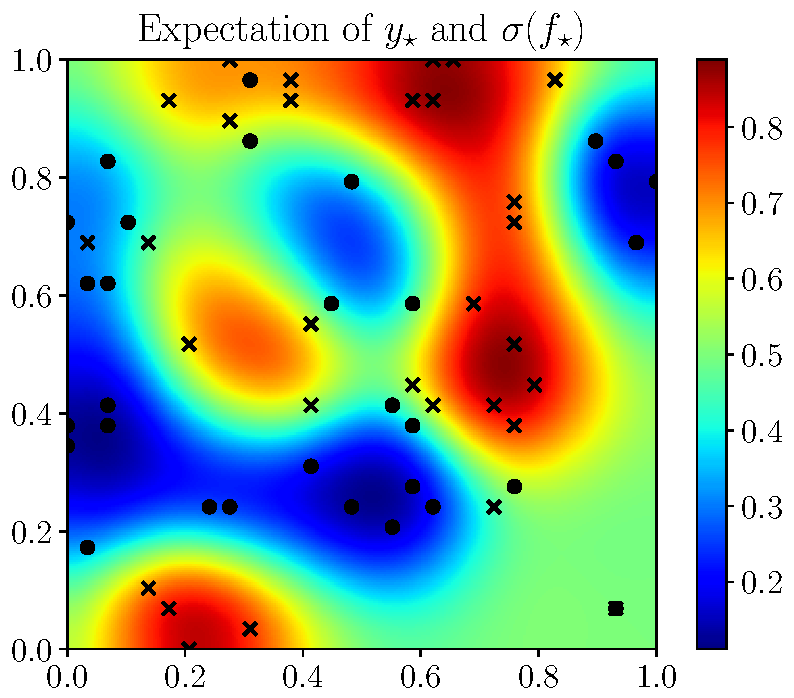
\includegraphics[width=.95\textwidth]{exp_y_star_cropped.pdf} \\
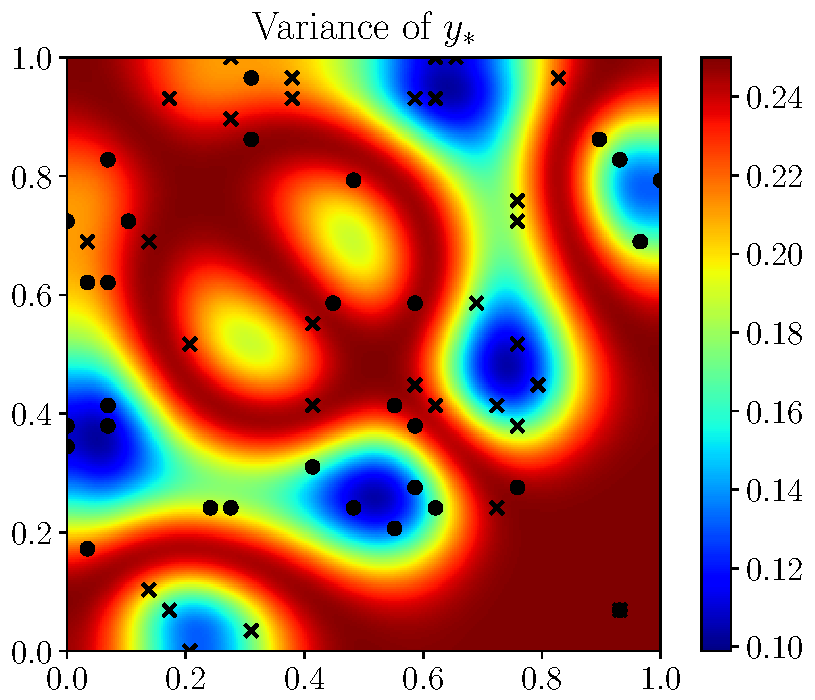
\includegraphics[width=.95\textwidth]{var_y_star_cropped.pdf} 
\end{minipage}
\end{frame}

\begin{frame}{Dueling-Thompson Sampling (DTS)}
\begin{minipage}{0.65\textwidth}
\begin{itemize}
\item To balance exploration \& exploitation, we borrow the idea of Thompson sampling by drawing a sample from the surrogate model.
\item Compute the \emph{soft-copeland} score on the drawn sample.
\item The value $\inputVector_{next}$ that gives the maximum \emph{soft-copeland} score gives a good balance between exploration and exploitation.
\item Take it as the \emph{first} value of the next duel. 
\end{itemize}
\end{minipage}
%
\begin{minipage}{.3\textwidth}
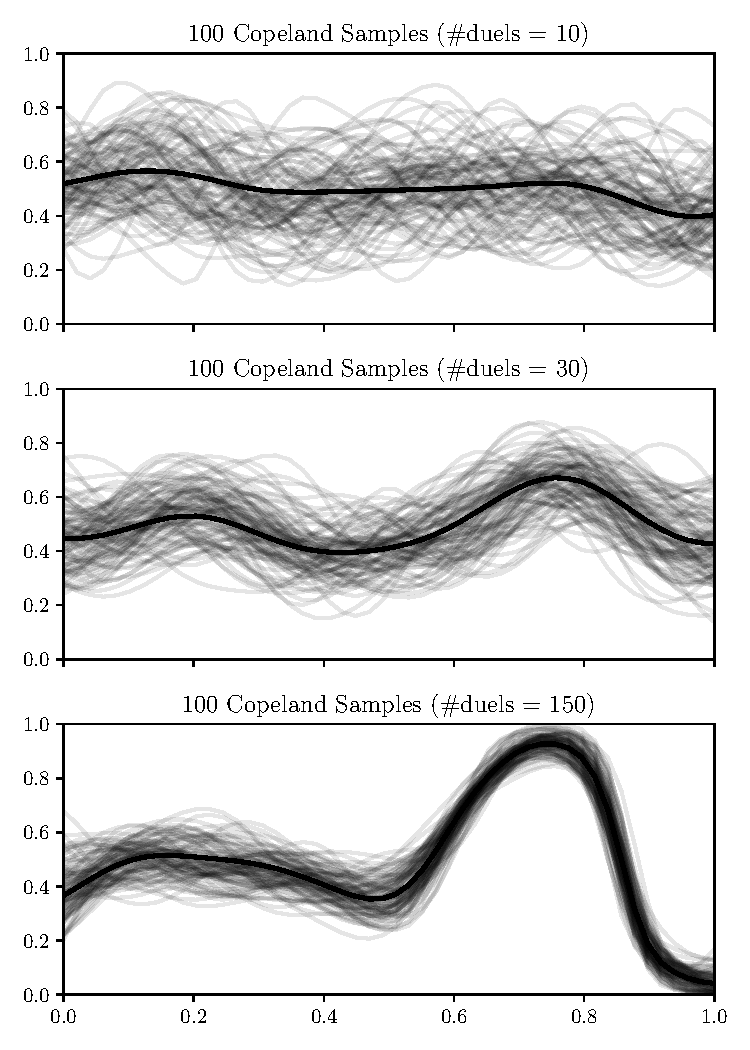
\includegraphics[height=0.9\textheight]{sample_multiple_copeland.pdf}
\end{minipage}
\end{frame}


\begin{frame}{Aleatoric Uncertainty \& Epistemic Uncertainty}
\begin{itemize}
\item The uncertainty of $y_\star$ comes from two sources: the \emph{aleatoric uncertainty} $\sigma(f_{\star})$ and the \emph{epistemic uncertainty} $p(f_{\star} | \dataSet, [\latentVector_{\star},\latentVector_{\star}'], \theta)$
$$p(y_{\star} = 1 | \dataSet,  [\inputVector,\inputVector'], \theta) 
= \int \sigma(f_{\star}) p(f_{\star} | \dataSet, [\latentVector_{\star},\latentVector_{\star}'], \theta) df_{\star} $$
\item Aleatoric Uncertainty: the stochasticity of the underlying process 
\item Epistemic Uncertainty: the uncertainty due to limited observations
\item Exploration should focus on \emph{epistemic uncertainty}.
\end{itemize}
\end{frame}


\begin{frame}{Multi-arm Bandits on 2D}
\centering
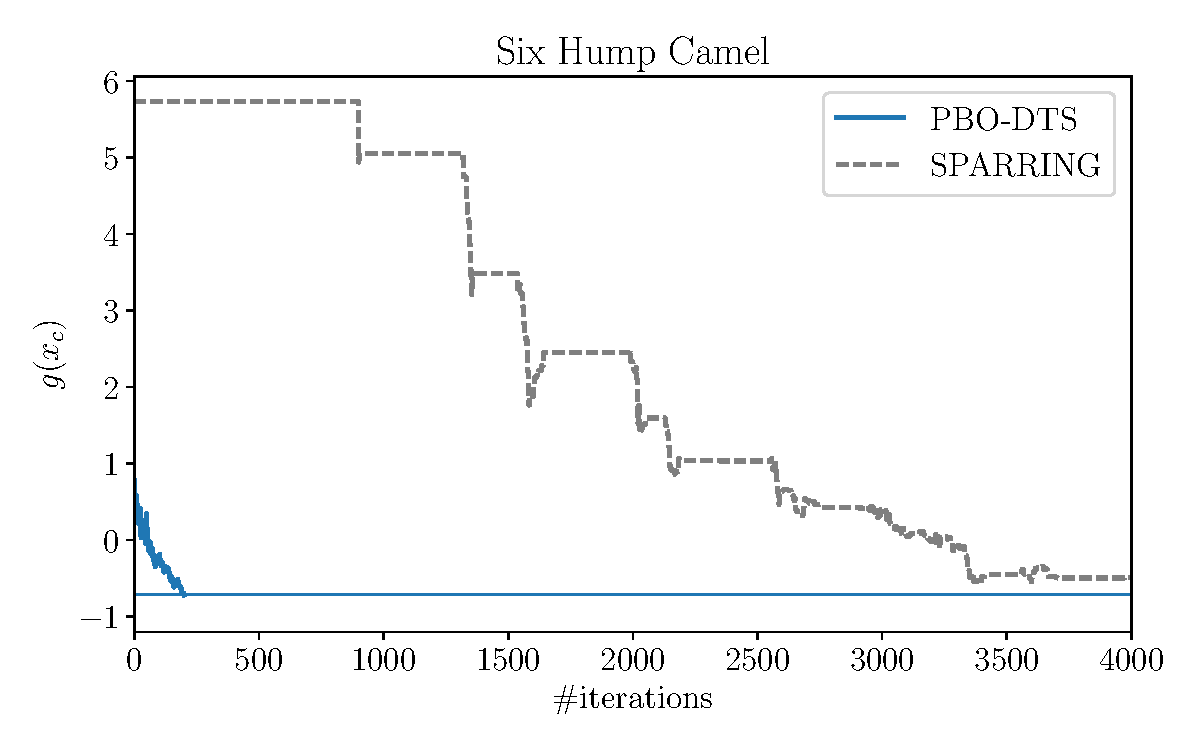
\includegraphics[width=0.6\textwidth]{results_sixhump_comparison.pdf}
\end{frame}

\bibliographystyle{plainnat}
{\footnotesize
\bibliography{bib_bopper}
}
%

\end{document}